\documentclass[12pt, a4paper]{report}
\usepackage[utf8]{inputenc}
\usepackage{float}
\usepackage{csquotes}
\usepackage[german]{babel}
\usepackage{hyperref}
\usepackage[onehalfspacing]{setspace}
\usepackage{geometry}
\usepackage{color}
\usepackage{listings}
\usepackage{graphicx}
\usepackage{acronym}
\usepackage{pgfplots}
%\usepackage{chngcntr}
%\counterwithout{figure}{chapter}
\usepackage{caption}
\DeclareCaptionFormat{citation}{%
   \ifx\captioncitation\relax\relax\else
     \captioncitation\par
   \fi
   #1#2#3\par}
\newcommand*\setcaptioncitation[1]{\def\captioncitation{\textit{Quelle:}~#1}}
\let\captioncitation\relax
\captionsetup{format=citation,justification=centering}
 
\usepackage{amsmath}
\usepackage{amssymb}

%\usepackage[normalem]{ulem}
%\useunder{\uline}{\ul}{}
\usepackage{lstautodedent}
\usepackage{dirtree}

\makeatletter
\newcommand{\sectionauthor}[1]{%
  {\parindent0pt\vspace*{-5pt}%
  \large{Author --- }
  \linespread{1.1}\large\scshape#1%
  \par\nobreak\vspace*{35pt} }
  \@afterheading%
}
\makeatother

\makeatletter
\newcommand{\chapterauthor}[1]{%
  {\parindent0pt\vspace*{-25pt}%
  \large{Author --- }
  \linespread{1.1}\large\scshape#1%
  \par\nobreak\vspace*{35pt} }
  \@afterheading%
}
\makeatother

\usepackage[backend=biber,
bibstyle=numeric, 
sorting=nty,
citestyle=authortitle-ibid,
natbib=true, 
hyperref=true,
isbn=true,
]{biblatex}
\addbibresource{lit.bib} 

\setcounter{secnumdepth}{3}
\setcounter{tocdepth}{3}
\geometry{
left=2.5cm,
right=2.5cm,
top=2.5cm,
bottom=2.5cm,
bindingoffset=5mm,
}
\definecolor{commentgreen}{RGB}{64, 128, 0}
\definecolor{stringred}{RGB}{179, 0, 0}
\definecolor{codebg}{RGB}{249, 248, 238}
\lstdefinestyle{custompython}{
	language=Python,
	backgroundcolor=\color{codebg},
	breaklines=true,
	commentstyle=\color{commentgreen},
	stringstyle=\color{stringred},
	keywordstyle=\color{blue},
	numbers=left,
	showstringspaces=false
}
\pagestyle{empty}
\begin{document}
%\documentclass[titlepage, 12pt]{scrbook}
%\usepackage[utf8]{inputenc}
%\usepackage[german]{babel}
%\usepackage{uarial}
%\usepackage{color}
%\renewcommand{\familydefault}{\sfdefault}
%\usepackage{fancyhdr}
%\usepackage{graphicx}
%\pagestyle{empty}
%\begin{document}
\begin{titlepage}
	\begin{flushleft}
	\begin{figure}
		\hspace*{-0,5cm}
		
\includegraphics[scale=0.25]{Bilder/DHBW_logo.jpg} \hspace*{5cm}
		
\includegraphics[scale=0.25]{Bilder/Atos_logo.png}
	\end{figure}
	\end{flushleft}
	\vspace*{-0.6cm}
	\begin{center}
	\textcolor{red}{Emotionsanalyse am Beispiel der Pokerfaceerkennung} \par \vspace*{0,5cm}
	Projektarbeit \par \vspace*{2cm}
	des Studienganges \textcolor{red}{Angewandte Informatik / Betriebliches Informationsmanagement}
	an der Dualen Hochschule Baden-Württemberg Mannheim \par \vspace*{1cm}
	von \par \vspace*{0,5cm}
	\textcolor{red}{Fabian Brandmüller, Maximilian Ludwig, Kevin Wrona} \par \vspace*{1cm}
	\today \par \vspace*{2cm}
	\begin{tabular}{l@{\hspace{3cm}}r}
		Bearbeitungszeitraum & \textcolor{red}{23.09.2019 - 24.04.2019} \\
		Betreuer der DHBW & \textcolor{red}{Prof. Dr. Eckhard Kruse} \\[1cm] 
	\end{tabular}
	\end{center}
\end{titlepage}
%\end{document}
\setlength{\parindent}{0em} 
\let\cleardoublepage\relax
\addtocontents{toc}{\protect\thispagestyle{empty}}
\addtocontents{lof}{\protect\thispagestyle{empty}}


\section*{Erklärung}
Wir versichern hiermit, dass die Studienarbeit mit dem Thema: \textcolor{red}{''Emotionsanalyse am Beispiel der Pokerfaceerkennung''} selbstständig verfasst und keine anderen als die angegeben Quellen und Hilfsmittel benutzt wurden.
\newline
\newline
\newline
\newline
---------------------------------------------       ------------------------------------------ \newline
Ort	\hspace{2cm}		Datum\hspace{3,5 cm}				    Unterschrift Fabian Brandmüller
\newline
\newline
\newline
---------------------------------------------       ------------------------------------------ \newline
Ort	\hspace{2cm}		Datum\hspace{3,5 cm}				    Unterschrift Maximilian Ludwig
\newline
\newline
\newline
---------------------------------------------       ------------------------------------------ \newline
Ort	\hspace{2cm}		Datum\hspace{3,5 cm}				    Unterschrift Kevin Wrona
\newpage
\section*{Abstract}
\sectionauthor{1329241}
Aufgabe dieser Studienarbeit ist es eine Emotionsanalyse durchführen zu können. Zur Veranschaulichung wird diese Thematik anhand des Anwendungsbeispiels der Pokerface-Erkennung realisiert.
Ziel ist es dabei, dass eine möglichst genaue Vorhersage der Emotionen gemacht werden kann, die es wiederum ermöglicht eine Aussage darüber zu treffen, ob eine Person ein Pokerface aufgesetzt hat, oder nicht.
Um dies umzusetzen wird eine künstliche Intelligenz entwickelt, genauer gesagt ein neuronales Netz. Die Trainings und Testdaten dieses Netzes sind dabei $35887 $ verschiedene Gesichtsbilder der FER (Facial Expression Recognition) Challenge von Kaggle. Analysiert werden die Emotionen ''Hapiness'', ''Sadness'', ''Fear'', ''Surprise'', ''Anger'', ''Neutral''. Mittels dieser Daten kann das trainierte Modell eine Genauigkeit in der Emotionsvorhersage von 55,71\% erzielen. die Rate der richtig erkannten Pokerfaces zu testen ist jedoch nicht so einfach, weshalb hierzu keine Daten in dieser Arbeit ermittelt wurden. Lediglich durch Ausprobieren ist es möglich die Genauigkeit der Pokerface-Erkennung festzustellen. Das Erkennen eines Pokerfaces ist mit der hier entwickelten Lösung jedoch möglich genauso wie eine Verwendung in der Praxis. 


\newpage
%\renewcommand*{\chapterpagestyle}{empty}
\renewcommand{\thefigure}{\Alph{chapter}.\Alph{figure}}
\renewcommand{\thetable}{\Roman{chapter}.\Roman{table}}

\tableofcontents
\listoffigures
\listoftables
\lstlistoflistings
\newpage
\chapter{Einleitung}
\chapterauthor{1329241}
\pagestyle{plain}
\setcounter{page}{1}
''Several researchers have stated that facial expression recognition appears to play one of the most important roles in human communication'' 
\footcite[Vgl.][1]{FaceRec}
Dieses Zitat von Katherine B. Leeland gibt einen Einblick in die Relevanz der Emotionserkennung für den Menschen. Fragen zu dieser Thematik stellen sich allerdings nicht erst seit Beginn der Digitalisierung. Bereits der Evolutionsforscher Charles Darwin
fragte sich, ob von den Gesichtsausdrücken einer Person nicht auch der emotionale Zustand abgeleitet werden kann.
\footcite[Vgl.][2]{FaceRec}
Einen solchen Zustand von einem Mitmenschen mittels Software abzulesen, ist jedoch nicht leicht zu realisieren. Bereits durch kleine Änderungen in der Mimik werden verschiedene Emotionen ausgedrückt. Zum Beispiel, indem eine Person bei Wut die Lippen zusammenpresst und die Augen zusammenkneift oder bei Trauer die Mundwinkel nach unten zieht.
\footcite[Vgl.][249]{HandbookFaceRec}
Durch derartige Ausdrücke können Emotionen wie Wut oder Trauer Ausdruck gewinnen.
Es gibt bereits Emotionserkennungssoftware, welche unter anderem in der Wirtschaft eingesetzt wird. Die Anwendungsgebiete reichen dabei von Jobinterviews, in denen analysiert wird, inwieweit die Bewerber für den jeweiligen Job geeignet sind,
\footcite[Vgl.][]{mixedArticle}
bis hin zur Automobilindustrie. Mittels geeigneter Sensorik wird dort versucht, die Emotion und somit den physiologischen Zustand des Autofahrers zu analysieren.
\footcite[Vgl.][Herausforderung]{Frauenhofer}
Diese Daten legen den Grundbaustein für Warnsysteme, welche den Fahrer darauf hinweisen können, dass sein Zustand zum Betrieb eines Kraftfahrzeugs ungeeignet ist. Solche Einsatzszenarien werden jedoch auch durchaus kontrovers diskutiert. Auf Kritik stößt unter anderem, dass die sogenannten ''Basisemotionen'' - z.B. Wut, Trauer, Ekel, Freude, Furcht, Überraschung - , die verwendet werden, um den KIs Emotionserkennung beizubringen, selbst umstritten sind.
\footcite[Vgl.][]{SZ}
Vor allem ethische Bedenken werden im Bezug auf die Anwendungsgebiete zunehmend geäußert. Denn je nach Emotion, die erkannt werden soll, liegt die Fehlerrate sehr hoch. So hat das Fraunhofer Institut, welches am Einsatz von Emotionserkennung in Fahrzeugen arbeitet, festgestellt, dass eine Emotionserkennung je nach Zielemotion eine Vorhersagekraft zwischen 6\% und 95\% haben kann.
\footcite[Vgl.][Ergebnis]{Frauenhofer}
Diese negativen Aspekte treffen jedoch nur teilweise auf das hier behandelte Forschungsprojekt zu, wie im Folgenden dargelegt werden soll:
Basierend auf den zuvor genannten Basisemotionen Wut, Frucht, Trauer, Freude und Ekel soll in dieser Arbeit getestet werden, inwieweit eine technische Vorhersage der Emotionen mittels künstlicher Intelligenz möglich ist. Dies erfolgt am Anwendungsbeispiel der Pokerface-Erkennung. Mittels der hier entworfenen technischen Lösung soll daher getestet werden, inwiefern ein noch zu definierendes Pokerface erkannt werden kann. Diese Forschungsarbeit hat also das Ziel, Emotionen so genau wie möglich zu analysieren und durch geeignete Algorithmen zu ermitteln, ob ein Pokerface vorhanden ist oder nicht. Der aus dieser Arbeit hervorgehende Prototyp ist dabei jedoch theoretisch gesehen nicht an das hier verwendete Fallbeispiel des Pokerspielens gebunden. Die Grundidee dieses Prototypen lässt einige hypothetische Einsatzszenarien in der Praxis zu. Diese haben eine gewisse Schnittmenge mit denen von ''normaler'' Emotionserkennungssoftware, jedoch gibt es auch einige weitere. Im Folgenden werden
einige denkbare Szenarien expliziert:
\begin{itemize}
	\item{Polizeiverhöre}
\end{itemize}
Es ist denkbar, dass eine erweiterte Form des entwickelten Prototypen bei Polizeiverhören eingesetzt werden könnte. Hierdurch könnten Beamte die Anwendung eines Pokerfaces durch den Beschuldigten erkennen, was auf eine Lüge hinweisen würde. Neben der gebräuchlichen Verwendung eines Lügendetektors wäre der Einsatz, der in dieser Arbeit erstellten Lösung, eine kostengünstige Variante.
\begin{itemize}
	\item{Gerichtsverhandlungen}
\end{itemize}
Das zweite Einsatzgebiet ist ähnlich zu dem Ersten. Bei Gerichtsverhandlungen gelten die gleichen Voraussetzungen wie bei einem Verhör der Polizei. Zwar müssen die Vorgeladenen eine eidesstattliche Erklärung abgeben, welche beinhaltet, nur die Wahrheit zu sagen, jedoch ist zu bezweifeln, ob dies auch immer der Fall ist.
Nun soll nicht der Eindruck entstehen, dass das hier gebaute Werkzeug ein Lügendetektor ist. Es ist ebenfalls nicht möglich, dass von einem Pokerface immer auf eine Lüge geschlossen werden kann. Jedoch ist ein Pokerface ein Zeichen dafür, dass sich diese Person ihren emotionalen Zustand nicht anmerken lassen möchte. Und dies wiederum deutet eher daraufhin, dass die Person nicht oder nur teilweise die Wahrheit sagt.
\begin{itemize}
	\item{Pokerspiel}
\end{itemize}
Wie bereits erwähnt, ist dieses Einsatzszenario das Fallbeispiel dieser Arbeit. Dies liegt unter anderem daran, dass der erste Begriff, der mit dem Wort Pokerface - bzw. einem emotionslosen Gesichtsausdruck - in Verbindung gebracht wird, das Pokerspiel selber ist. Und auch in diesem kann es nützlich sein zu wissen, ob die Kontrahenten ein Pokerface aufsetzen oder nicht. Denkbar wäre es, dass ein Mitspieler zum Beispiel mittels einer Kamera das Gesicht des Gegenübers scannt und analysiert, ob ein Pokerface vorliegt oder nicht. Aufgrund der gewonnenen Erkenntnis kann er dann entsprechend reagieren.

\chapter{Anforderungen}
Das nun folgende Kapitel thematisiert die konkrete Aufgabenstellung der Arbeit sowie eine Anforderungsanalyse mittels MoSCoW-Priorisierung. 

\section{Aufgabenstellung}
\sectionauthor{1329241}
Das Projekt selber wird an der DHBW in Mannheim unter der Betreuung von Prof. Dr. Eckhard Kruse durchgeführt. Wie eingangs erwähnt, soll mittels künstlicher Intelligenz erkannt werden, welche Emotion vorliegt. Zur Umsetzung dieser Aufgabe wird eine Bilderkennungssoftware angefertigt, welche ein übermitteltes Bild anhand vorhandener Emotionen analysiert. Sollte durch die Software keine Emotionsänderung erkannt werden, wird dem Anwender das Vorhandensein eines Pokerfaces zurückgegeben. Wie bereits in der Einleitung beschrieben, sind diverse Einsatzmöglichkeiten vorhanden, an die das Werkzeug leicht angepasst werden kann.

\section{Usecase}
\sectionauthor{1329241}
Wie bereits erwähnt, ist der hier behandelte Use Case das Pokerspiel selber. An diesem soll ermittelt werden, inwieweit sich Emotionen oder das Abhandensein von Emotionen vorhersagen lassen. Dieses Fallbeispiel wurde gewählt, da es unter anderem das Naheliegendste ist und ein simples und leicht zu konstruierendes Szenario impliziert. Dabei soll mithilfe einer Kamera ein Bild von einem Pokerspieler aufgenommen werden und dann mittels dem hier entworfenen Prototypen verarbeitet und analysiert werden. Am Ende soll dann eine Vorhersage der Emotionen getätigt werden, die dem Photographen zur Verfügung gestellt wird.


\section{MoSCoW Priorisierung}
\sectionauthor{1329241 - 8774695 - 2356667}
Diese Arbeit soll methodisch mit der MoSCoW-Priorisierung bearbeitet werden. Diese Art der Priorisierung teilt die zu bearbeitenden Anforderungen in vier Kategorien ein:
\footcite[vgl.][90]{Projektmanagement}
\begin{itemize}
\item Must - Core Anforderungen, die unbedingt umgesetzt werden müssen
\item Should - Anforderungen, die ebenfalls umgesetzt werden müssen, jedoch im Nachhinein noch durch Change Requests verändert werden können
\item Could - Anforderungen, die nach den Must und Should Anforderungen umgesetzt werden sollen, sofern noch Ressourcen und Zeit vorhanden sind, um diese zu bearbeiten
\item Won't - Anforderungen, die nicht in diesem Projekt bzw. Release erfolgen, jedoch in einer zukünftigen Version bearbeitet werden können 
\end{itemize}
Im Zuge des Projektes wurden die vorhandenen Anforderungen anhand der MoSCoW-Priorisierung wie folgt eingeordnet:
\begin{itemize}
\item Must
\begin{itemize}
\item Emotionen werden nicht zufällig erkannt
\item Es wird zwischen Pokerface und kein Pokerface unterschieden
\item Benutzerfreundliche Interaktionsmöglichkeit, um Input zu liefern und Output darzustellen
\end{itemize}
\item Should
\begin{itemize}
\item Die Genauigkeit zur Erkennung der richtigen Emotion soll über 50\% liegen
\item Es sollen mindestens fünf verschiedene Emotionen erkannt werden
\item Die Erkennung einer Emotion und eines Pokerfaces soll innerhalb des Pokerspielzuges eines Spielers (ca. 20 Sekunden) erfolgen
\end{itemize}
\item Could
\begin{itemize}
\item Die Emotionen aus Bildern können nahezu in Echtzeit analysiert werden
\item Das Trainieren des Modells kann innerhalb eines Arbeitstages erfolgen
\item Eine Oberfläche zur intuitiven Bedienung der Lösung ohne technisches Verständnis muss vorhanden sein
\end{itemize}
\item Won't
\begin{itemize}
\item Neben dem Analysieren von Bildern ist auch die Analyse von Videos möglich
\item Das Modell soll bei jeder Belichtung valide Ergebnisse liefern
\end{itemize}
\end{itemize}
Dabei sollen die einzelnen Anforderungen entsprechend ihrer Priorität abgearbeitet werden. So kann am Ende der Erfolg der Arbeit deutlich besser eingeordnet werden.

\let\cleardoublepage\relax

\chapter{Stand der Technik}
\chapterauthor{1329241}
In diesem Abschnitt soll der aktuelle Forschungs- und Entwicklungsstand im Bereich Emotionserkennung thematisiert werden. Jedoch muss dafür erst einmal eine Unterscheidung der Begrifflichkeiten Emotionserkennung und Gesichtserkennung erfolgen, da beide Gebiete Überschneidungen haben, jedoch inhaltlich und von ihren Zielen verschieden sind. Innerhalb dieser Arbeit wird sich beiden Themenbereichen bedient, weshalb zumindest eine grobe Erläuterung der Vorgehensweise dieser Ansätze sinnvoll ist.

\section{Gesichtserkennung}
\sectionauthor{1329241}
Gesichtserkennung ist eine Disziplin der Informatik in der es darum geht Gesichter wieder zu erkennen, und gegebenenfalls verschiedenen Personen zuzuordnen. Dabei lässt sich der Prozess der Gesichtserkennung in vier Phasen einteilen, Face ''detection'', ''alignment'', ''feature extraction'' und ''matching'', wie anhand von Grafik \ref{fig:Face Recognition} sichtbar ist.
\footcite[Vgl. ][2]{HandbookFaceRec}
\begin{figure}[h]
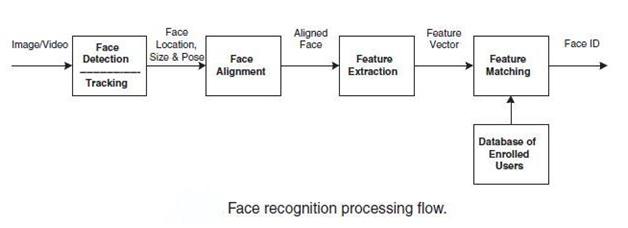
\includegraphics[width=\linewidth]{Bilder/FaceRecognition.png}
\setcaptioncitation{ https://alitarhini.files.wordpress.com/2010/12/untitled1.png}
\caption{ Phasen der Gesichtserkennung}
\label{fig:Face Recognition}
\end{figure}
Die Detection Phase ist dafür verantwortlich, zu erkennen, ob Gesichter vorhanden sind in einem Bild oder aber Video.
\footcite[Vgl. ][2]{HandbookFaceRec}
In der darauffolgenden Alignment-Phase hingegen wird die Lokalisierung der Gesichter genauer, indem Gesichtskomponenten wie Augen, Augenbrauen, oder die Nase genauer lokalisiert werden. Dabei wird das Bild oder Video ebenfalls normalisiert, indem z.B. die Bildbeleuchtung angepasst wird.
\footcite[Vgl. ][2]{HandbookFaceRec}
In der Feature extraction hingegen werden die verschiedenen Gesichtskomponenten wie Augen, Nase, Mund, dem Bild oder Video entnommen. Dies ist ein wichtiger Schritt für weitere Prozesse wie Eye Tracking oder Face Tracking. Alternativ kann sogar eine bestimmte Person anhand der extrahierten Merkmale erkannt werden.
\footcite[Vgl. ][Abstract]{IEEE}
In der letzten Phase, dem Matching, geht es darum, die gewonnen Daten mit den in der Datenbank vorhandenen Gesichtern abzugleichen. Wenn eine genügende Übereinstimmung gefunden wurde, wird ein Match mit einer Person ausgegeben.
\footcite[Vgl. ][3]{HandbookFaceRec}
Die Anwendungsgebiete von Software, die Gesichtserkennung ermöglicht, sind mannigfaltig. Sie reichen von Applikationen die ein Gerät wie ein Smartphone entsperren, wenn das Gesicht des Besitzers als Treffer ausgegeben wurde, bis hin zur Anwendung in Verbrechensbekämpfung. In jedem dieser Szenarien wird dabei der oben beschriebene Ablauf durchgegangen und abhängig vom zu liefernden Ergebnis eine Abschlussaktion vorgenommen.

\section{Emotionserkennung}
\sectionauthor{1329241}
In diesem Unterkapitel nun sollen Emotionen an sich thematisiert werden, da diese maßgeblich sind für das zu entwickelnde Tool. Eine Definition von Emotionserkennung ist per se nicht schwer zu geben. Prinzipiell beschäftigt sich Emotionserkennung mit der Analyse von Gesichtern und den Emotionen, die diese Gesichter darstellen. Jedoch ist der Begriff der Emotionen nicht ganz so einfach zu definieren, wie im Folgenden erläutert wird: 

%\begin{itemize}
%\item was ist Emotionserkennu
%\item usecase für emotion recognition
%\item Aiusblick und Kontroverse
%\end{itemize}

\subsection{Emotionen}
\sectionauthor{1329241}
%\begin{itemize}
%\item Def. von Emotionen
%\end{itemize}
Grundsätzlich gibt es verschieden Ansätze Emotionen zu definieren und einzuteilen. Eine Variante ist dabei die eingangs erwähnte, nicht ganz unumstrittene Einteilung in Basisemotionen. Eine gängige Einteilung ist dabei die verschiedenen Emotionen in acht Bereiche einzuteilen. Diese Einteilunge wurde 1984 von Plutchik postuliert und beinhaltet die Emotionskategorien Angst, Wut, Freude, Trauer, Akzeptanz, Ekel, Erwartung und Überraschung.
\footcite[Vgl. ][3]{FaceRec}
Jedoch ist dies nicht die einzige mögliche Einteilung. Als weiteres Beispiel teilt MacLean die Emotionen in lediglich sechs Kategorien ein, welche da wären: Verlangen, Wut, Angst, Niedergeschlagenheit, Freude und Zuneigung.
\footcite[Vgl. ][3]{FaceRec}
Wie sich bereits an den beiden Beispielen zeigt, geht die Meinungen der Forscher dabei stark auseinander, welche und wie viele Emotionen zu den sogenannten ''Basis Emotionen'' gehören. In dieser Arbeit werden die Emotionen in sechs Kategorien eingeteilt, in Wut, Verachtung, Angst, Freude, Trauer, Überraschung und Neutral. Diese Einteilung entspricht an sich keiner gängigen Einteilung, jedoch wurde diese aus den folgenden Gründen gewählt: \newline
Die hier genannten Emotionen lassen sich gut anhand von Bildern erlernen, da diese zum Teil komplementär und somit eindeutig sind. Es ist aber auch einfacher Testdatensätze zu bekommen für ein
freudiges Gesicht oder ein überraschtes, als ein Gesicht mit dem emotionalen Ausdruck Akzeptanz. Zudem sind die gewählten Emotionen häufig bei dem Test Usecase dieser Arbeit anzutreffen, dem Texas Hold'em Poker.

\subsection{Abgrenzung zur Gesichtserkennung}
\sectionauthor{1329241}
Der grundlegende Unterschied zwischen Emotions- und Gesichtserkennung liegt nun darin, dass bei der Emotionserkennung selber nicht die agierende Person im Vordergrund steht, sondern die Aktion die sie ausführt. Bei der Gesichtserkennung hingegen spielt lediglich die Rolle wer eine Aktion ausführt und ob es einen Treffer in der Datenbank gibt, oder nicht. Wegen dieser Unterschiede ist auch die technische Realisierung eines Prototypen, vor allem im Bezug auf die Architektur,  durchaus unterschiedlich. Dies ist jedoch ebenso von den unterschiedlichen Anwendungsszenarien der beiden Verfahren bedingt.
Denn diese sind ebenso verschieden. Während Gesichtserkennung eher in den Bereich IT-Security oder aber Social Media (Snapchat Filter) eingesetzt wird, ist Emotionserkennung eher Informationsgenerierend.
Zum Beispiel können durch Emotionserkennung Informationen zugänglich werden, wie das Befinden eines Individuums ist, ob es emotional betroffen ist, oder aber nicht emotional betroffen wirken möchte und ein Pokerface aufsetzt.
Wegen dieser signifikanten Unterschiede kann daher trotz der Gemeinsamkeiten nicht gesagt werden, dass Emotionserkennung eine Unterkategorie von Gesichtserkennung ist.

\section{Wann ist ein Gesicht ein Pokerface?}
\sectionauthor{1329241}
\label{pokerface}
Bis zu diesem Teil der Arbeit wurde schon immer wieder das Wort Pokerface verwendet ohne es formal zu definieren. Jedoch ist es für die Arbeit wichtig, eine konkrete Definition für diesen Begriff zu geben, da ansonsten die Anforderungen an die Arbeit nicht korrekt bewertet werden könnten. Da es mehrere Ansätze gibt ein Pokerface zu definieren, wird dies in diesem Abschnitt nachgeholt. Zum einem gibt es den trivialen Ansatz, dass ein Pokerface dann vorliegt, wenn ein Subjekt keinerlei Emotion in seinem Gesicht zu erkennen gibt. Dies würde einer neutralen Emotion entsprechen. Dieser Fall kann auch vergleichsweise einfach behandelt werden, da diese neutrale Emotion auch in die Basisemotionen mit aufgenommen wurde in dieser Arbeit. Das bedeutet, dass beispielsweise ein neuronales Netz auch diese Arten von Gesichtern klassifizieren könnte. \newline
Der zweite Ansatz ist weniger intuitiv, jedoch ebenso wichtig. Es kann durchaus angenommen werden, dass z.B. ein sehr erfahrener Pokerspieler weiß, dass man ein Pokerface einfach identifizieren kann, und demnach alleine dadurch Informationen gewinnen kann. Um dem entgegenzuwirken könnte ein solcher Spieler eine andere Art Pokerface verwenden. Es wäre denkbar, dass er versucht sein Gesichtsausdruck permanent gleich zu halten, indem er eben dauerhaft lacht oder lächelt, dauerhaft betrübt, wütend, ängstlich, etc. aussieht. Dieser Ansatz ist weniger intuitiv als der erste und könnte demnach auch weniger schnell erkannt werden. Im Verlaufe der Arbeit wird mit der zweiten Definition gearbeitet.

\section{Emotionserkennung mithilfe von Deep Learning}
\sectionauthor{8774695}
In dem nun folgenden Kapitel wird erörtert, wie das Ziel des Prototypen dieser Arbeit - das Erkennen eines Pokerfaces - mittels eines neuronalen Netzes umgesetzt werden kann. Dabei wird weniger auf die generellen Eigenschaften von neuronalen Netzen Bezug genommen, als auf die in dieser Arbeit spezifischen Aspekte. Diese sind vor allem verschiedene Ansätze und Möglichkeiten mittels Machine Learning eine Emotionserkennungssoftware zu erstellen.

\subsection{Machine Learning - Frameworks}
\sectionauthor{8774695}
Um die gegebene Aufgabenstellung der Erkennung von Emotionen mittels der Analyse eines Gesichtes umsetzen zu können, musste ein entsprechendes Framework Anwendung finden, welches den Anforderungen gerecht wird. Maschinelles Lernen gehört in der heutigen Softwareentwicklung zu den beliebtesten Themen, wodurch dieses schnelle, regelmäßige Änderungen und Weiterentwicklungen erfährt. Dementsprechend werden auf dem Markt auch zahllose kostenlose wie auch kostenpflichtige Frameworks angeboten. Darunter fallen unter anderem
 OpenCV, Tensorflow oder Pandas. Möchte man nun das geeignete Framework für das eigene Projekt ausfindig machen, muss man das gegebene Angebot nach einigen Kriterien filtern. Als erstes stellt sich die Frage, was für eine Art von Applikation man umsetzen möchte. Soll das Projekt Texte analysieren oder wie im Falle dieses Projektes die Emotionen aus einem gegebenen Bild? Welche Programmiersprache wird innerhalb des Projektes eingesetzt? Zudem sind Informationen zur Lizenz und dem Support wichtig, sowie insbesondere die Community.\newline
Nach entsprechender erster Selektion musste sich schlussendlich zwischen Dlib und Keras entschieden werden, welche für die Umsetzung der Anforderungen dieses Projektes am besten geeignet schienen. Beide Frameworks werden in den folgenden beiden Unterkapitel dem Leser kurz vorgestellt und anschließend wird ein Fazit gezogen, welches der beiden für dieses Projekt am geeignetsten ist.

\subsubsection{Dlib}
\sectionauthor{8774695}
Dlib ist nach dessen Entwickler Davis King ein modernes C++ Toolkit, welches Machine-Learning Algorithmen und Tools zur Entwicklung komplexer Software enthält, um Probleme aus der echten Welt lösen zu können.\footcite[Vgl.]{netguru}
\newline
Dlib selbst wurde in der Programmiersprache C++ entwickelt und kann durch eine Anbindung auch für Python Projekte eingesetzt werden. Die Software-Bibliothek kann unter den Bedingungen der Boost-Lizenz frei genutzt werden und ist durch entsprechende APIs des jeweiligen Betriebssystems plattformunabhängig. Ein weiterer Vorteil bietet die Unabhängigkeit der Bibliothek von anderen Bibliotheken. %Von Wikipedia (Vlt. andere Quelle suchen)
Dlib ist seit dem Jahr 2002 in Entwicklung und bietet dementsprechend unzählige Features an, welche für verschiedenste Einsatzgebiete verwendet werden können, wie numerische und graphische Modell-Algorithmen und vor allem Gesichtserkennung.\footcite[Vgl.][]{netguru}
Eines der größten Vorteile dieser Bibliothek besteht in der ausführlichen Dokumentation für sämtliche Klassen und Funktionen, wie es nicht häufig der Fall ist für vergleichbare Open-Source Projekte.\footcite[Vgl.]{Dlib}

\subsubsection{Keras}
\sectionauthor{8774695}
Die Open-Source Bibliothek Keras wurde im Vergleich zu Dlib im Jahre 2015 von dem Google-Programmierer François Chollet in der Programmiersprache Python entwickelt.\footcite[Vgl.][]{Keras}
Das ursprüngliche Ziel von Keras war es eine Abstraktionsschicht für das Framework Theano zu bilden, um die Handhabung zu vereinfachen. Mit der Veröffentlichung von TensorFlow im November 2015 wurde Keras im folgenden Monat weiter entwickelt um auch TensorFlow als Backend verwenden zu können. Schlussendlich konnte Keras die Frameworks TensorFlow, Theano und das Microsoft Cognitive Toolkit (kurz: CNTK) einbinden und beliebig austauschen.\footcite[Vgl.][]{Keras3} Allerdings stoppte im September 2017 die Weiterentwicklung an Theano
\footcite[Vgl.][]{Theano}
 waraufhin Keras zunehmend an TensorFlow gebunden wurde.\footcite[Vgl.][]{Keras4} Schlussendlich wurde mit Keras 2.3, welches im September 2019 veröffentlicht wurde, die multi-backend Version eingestellt.\footcite[Vgl.][]{Keras5} Aus diesem Grund wird Keras überwiegend mit dem Framework TensorFlow verwendet.
\newline
Bei der Entwicklung von Keras stand die Benutzerfreundlichkeit als eines der wichtigsten Prinzipien im Mittelpunkt. Dem gefolgt bietet Keras eine schnelle und leichte Erstellung neuronaler Netze. Durch ein ausführliches Feedback können Fehler durch den Benutzer schnell ausfindig gemacht und behoben werden. Ein weiteres Designprinzip von Keras ist die Modularität, mithilfe derer man verschiedene Module beliebig konfigurieren und miteinander kombinieren kann. Zudem bietet die Open-Source Bibliothek die Unterstützung von rekurrenten und konvolutionalen Netzwerken, sowie die Unterstützung der GPUs und CPUs, was für die Umsetzung dieses Projektes von Vorteil ist.\footcite[Vgl.][]{Keras2}
Zuletzt steht hinter Keras eine große aktive Community, welche zahlreiche Tutorials und Hilfestellungen für verschiedenste Problemstellungen liefert.


\subsubsection{Unterschiede}
\sectionauthor{8774695}
Zusammenfassend kann gesagt werden, dass Dlib eine mächtige Bibliothek für die Umsetzung verschiedenster Aufgaben ist. Die ausführliche Dokumentation bietet eine große Hilfestellung. Jedoch folgt aus dem Angebot der zahlreichen Features auch eine längere Einarbeitung, bis die Anforderungen produktiv umgesetzt werden können.\newline
Keras hingegen bietet durch dessen benutzerfreundliche Entwicklung und den zahlreichen Tutorials eine schnelle erste Umsetzung der Aufgaben. Durch die Modularität und der aktiven Community können viele öffentliche Lösungen genutzt und für die eigenen Bedürfnisse abgeändert werden. 
Aus diesem Grund und aufgrund der Unterstützung der rekurrenten und konvolutionalen Netzwerken wurde sich für die Verwendung von Keras als Open-Source Bibliothek in diesem Projekt entschieden.


\subsection{Supervised vs. Unsupervised Learning}
\sectionauthor{1329241}
In diesem Abschnitt werden die beiden Ansätze des Supervised bzw. des Unsupervised Learnings evaluiert. Dabei sollen jedoch beide Begriffe nicht noch ausführlich beleuchtet werden. Es ist lediglich zu erwähnen, dass Supervised Learning Algorithmen im Gegensatz zu Unsupervised mit Datensätzen arbeiten, die kategorisiert sind. Damit ist es ihnen möglich Bilder die eingegeben werden anhand dieser Kategorien zu klassifizieren. Grundlegende Informationen zu den einzelnen Vorgehensweisen können aus den hier zitierten Büchern entnommen werden.  
\footcite[Vgl. ][]{Supervised}
\footcite[Vgl. ][]{Unsupervised}
Nun gilt es zu klären, ob sich für die zugrundeliegende Aufgabe ein Supervised oder Unsupervised Ansatz eher anbietet. Ein Unsupervised Learning Algorithmus würde sich vor allem anbieten, wenn Zusammenhänge zwischen einzelnen Datensätzen gefunden werden sollen, die vielleicht nicht von Anfang an bekannt oder bewusst sind.
\footcite[Vgl. ][21]{Unsupervised}
Supervised Learning Algorithmen hingegen bieten sich vor allem an, wenn es darum geht einen Prozess zu automatisieren oder aus der Wirklichkeit zu replizieren.
\footcite[Vgl. ][4]{Supervised}
Das in dieser Arbeit zugrundeliegende Problem ist demnach vor allem für Supervised Learning Algorithmen geeignet. Dies liegt zum einem daran, dass jedem Bild eines Menschen eine Basisemotion zugeordnet werden kann. Zum anderen ist auch der verwendete Datensatz, mit dem das Modell trainiert und getestet werden soll, ebenfalls gelabelt. Deshalb bietet sich dieses Verfahren am meisten an. Es wäre auch hypothetisch denkbar, einen Unsupervised Learning Algorithmus zu verwenden, aber dieser Ansatz wäre suboptimal verglichen mit einem Supervised Algorithmus.

\subsection{Aktivierungsfunktion}
\label{Aktivierungsfunktion}
\sectionauthor{8774695}
Im Folgenden wird kurz auf die sogenannten Aktivierungsfunktionen eines neuronalen Netzwerkes eingegangen.
Dabei wird dem Leser lediglich eine kurze Einführung gegeben, weshalb diese Funktionen für Machine Learning verwendet werden sollten und weniger auf die dahinterliegende Mathematische Problemstellung, welche den Komplexitätsrahmen dieser Arbeit überschreiten würde.
\newline
Aktivierungsfunktionen werden für ein kompliziertes nichtlineares Zuordnen der Eingangsdaten und deren abhängigen Ergebnisse verwendet. In der einfachsten Mathematischen Darstellung kann man sich also die Eingangsdaten \textbf{X} und deren Gewichtung \textbf{W} vorstellen, auf welchen die Aktivierungsfunktion \textbf{f(x)} angewendet wird. Sollte bei der Berechnung eines neuronalen Netzes die Aktivierungsfunktion nicht explizit bestimmt werden, wird die einfachste Lineare Funktion \textbf{f(x)=x} verwendet, welche von ihrer Komplexität derart begrenzt ist, dass kein komplexes Funktionsmapping aus den Daten erlernbar ist. Daraus folgt, dass ein neuronales Netzwerk ohne Aktivierungsfunktion keine komplizierten Datenarten, wie zum Beispiel Bilder nutzen kann, welche für die Umsetzung der Aufgabe natürlich verwendet werden müssen.\footcite[Vgl.][]{Aktivierungsfunktion}
\newline
Welche Aktivierungsfunktion soll also eingesetzt werden? Die beliebtesten und bekanntesten Aktivierungsfunktionen sind \textit{Sigmoid}, \textit{Logistik}, \textit{Tanh (Hyperbolischer Tangens)}, sowie \textit{ReLu (Rectified Linear Unit)}.
Ein gemeinsames Problem der ersten drei genannten Funktionen liegt in dem sogenannten \textit{\textbf{Gradientenverschwinden}}, welches bei der ReLu Funktion vermieden und korrigiert wird. Auf das Problem des Grandientenverschwindens wird aufgrund dessen Mathematischer Komplexität nicht weiter eingegangen.In der Grafik \ref{fig: ReLu} ist der Funktionsgraph der ReLu Funktion dargestellt.
\begin{figure}[H]
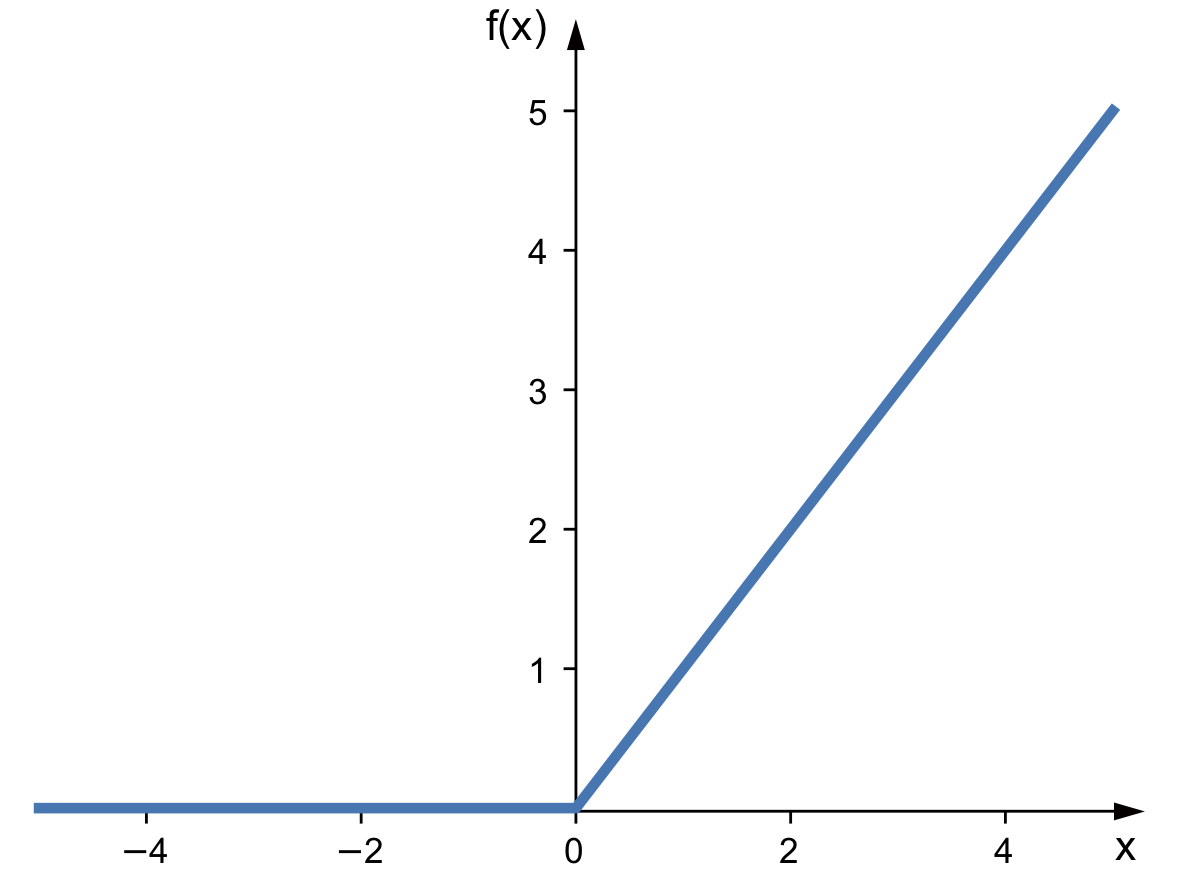
\includegraphics[width=\linewidth]{Bilder/relu.png}
\setcaptioncitation{https://sebastianraschka.com/images/faq/relu-derivative/relu\_3.png}
\caption{ReLu Funktionsgraph}
\label{fig: ReLu}
\end{figure}
Zu sehen ist die einfache mathematische Funktion der Form \textbf{ReLu(x) = max(0,x)}, welche für alle Eingabewerte \textbf{x $<$ 0 = 0} ausgibt, und für \textbf{x $>$ 0} einen einfachen linear steigenden Graphen darstellt. Aufgrund der einfachen und effizienten mathematischen Grundform, sowie der Fähigkeit des Umgehens des Gradientenverschwindens, wurde diese Aktivierungsfunktion immer beliebter und wird neuerdings in fast allen neuronalen Netzwerken verwendet.\footcite[Vgl.][]{Aktivierungsfunktion2}
\newline
Aus diesen Gründen wurde sich auch dafür entschieden diese Aktivierungsfunktion für das hier entwickelte Modell zu verwenden.

\section{Gesichtserkennung mit OpenCV}
\sectionauthor{1329241}
In dem nun folgenden Abschnitt wird der theoretische Aspekt der Gesichtserkennung mit dem Tool OpenCV erläutert. In der Arbeit findet die Gesichtserkennung an mehreren Stellen Anwendung, auch wenn es eigentlich um Emotionserkennung geht. So wird zum Beispiel, bevor eine Vorhersage über eine Emotion zu einem Bild gemacht wird, überhaupt erst geprüft, ob auf dem Bild auch ein Gesicht vorhanden ist. Dies ist auch notwendig, da dies die Fehlerbehandlung erleichtert. Sollte ein Bild eingegeben werden, auf dem kein Gesicht zu erkennen ist, darf auch kein Rückgabewert von Emotionsklassifizierungen erhalten werden, weshalb vorher überprüft werden sollte, ob ein menschliches Gesicht auf dem Bild vorhanden ist.

\subsection{Opencv Klassifizierer}
\sectionauthor{1329241}
OpenCV stellt verschiedenste Klassifizierer für die Aufgabe der Gesichtserkennung zur Verfügung. Zum einem die sogenannten HAAR-Cascade Klassifizierer, zum anderen dedizierte Gesichtserkennungsalgorithmen. Beide Arten werden im Laufe dieser Arbeit verwendet werden, weshalb es zum besseren Verständnis der Arbeit dienlich ist, die Funktionsweise dieser zu beleuchten.

\subsubsection{HAAR Cascade Klassifizierer}
\sectionauthor{1329241}
Als Datengrundlage für diese Art der Klassifizierer werden positive Bilder gebraucht - im Falle der Gesichtserkennung also Bilder mit Gesichtern - aber auch negative. Aus diesen werden dann Eigenschaften extrahiert und verarbeitet. Grundsätzlich ist diese Art der Klassifizierung deutlich flexibler als ''reine'' Gesichtserkennungsalgorithmen. Dies liegt daran, dass HAAR Klassifizierungen nicht auf Gesichter beschränkt sind, sondern auf zahlreiche Eigenschaften wie Augen und Münder oder gänzlich auf andere Objekte wie Mäuse und Häuser angewendet werden können. Ein HAAR-Cascade Klassifizierer lässt sich dabei in vier Bereiche einteilen.
\begin{itemize}
\item HAAR feature selection
\item Creating Integral Images
\item Adaboost Training
\item Cascading Classifiers
\end{itemize}
\footcite[Vgl.][]{willberger}
In dem ersten Schritt werden sogenannte HAAR-Features festgelegt. Diese sind im Wesentlichen verschiedenartige Ausschnitte aus den Bildern. Eine beispielhafte Selektion dieser kann der Grafik \ref{fig: haar-features} entnommen werden.
\begin{figure}[h]
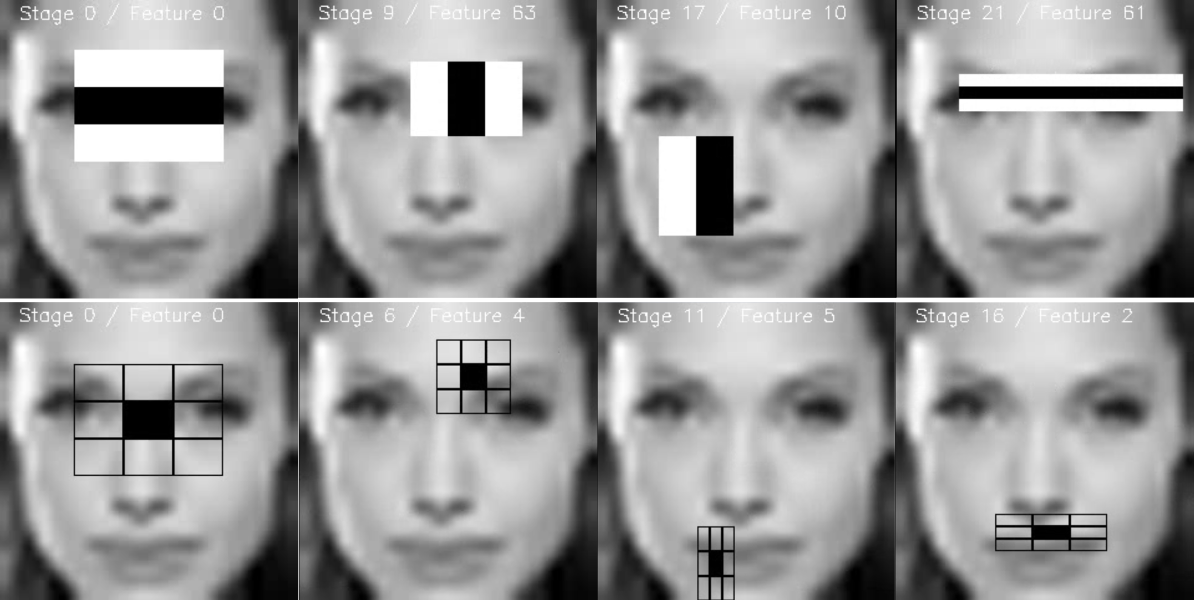
\includegraphics[width=\linewidth]{Bilder/haar-cascade.png}
\setcaptioncitation{ https://docs.opencv.org/master/dc/d88/tutorial\_traincascade.html}
\caption{haar features}
\label{fig: haar-features}
\end{figure}
Wie in der Grafik ebenfalls zu sehen ist, sind diese Features allesamt rechteckig. Dies bietet die Möglichkeit, die Berechnungen, die gemacht werden müssen, zu beschleunigen, indem Schritt zwei angewandt wird. die vorliegenden Bilder werden dabei in Integralbilder umgewandelt. Diese werden im Folgenden nicht genau expliziert, jedoch werden in Integralbildern, vereinfacht gesagt, in jedem Punkt des Bildes die Pixelsummen eines Rechteckes gehalten, das vom Ursprung bis zu dem jeweiligen Pixel aufgespannt wird. Bei einem Punkt (x,y) wird also das Rechteck (0,0), (x,0), (0,y), (x,y) betrachtet.
\footcite[Vgl.][]{integral}
Nun können verschiedene HAAR-Features selektiert werden. Das Problem dabei ist jedoch, dass diese für sich nicht sonderlich aussagekräftig sind. Beispielsweise ein Feature, dass die Nasenflügel betrachtet, ist nicht in der Lage ein Gesicht wirklich zu erkennen. Um deshalb ein aussagekräftiges Ergebnis zu erzielen, werden die besten dieser sogenannten schwachen Klassifizierer zu einem starken Klassifizierer zusammengefasst und trainiert. Dieser Schritt beschreibt das Adaboost-Training.
\footcite[Vgl.][]{willberger}
Diese Trainingsart benutzt nun den letzten Teil, das Kaskadieren von Klassifikatoren. Im Wesentlichen handelt es sich dabei um eine Methode, die so schnell wie möglich falsche Bilder, also solche die nicht der gewünschten Klasse entsprechen, aussortiert. Dabei wird in multiplen Stadien gearbeitet, in denen ein sich verschiebender Rahmen über das Bild gelegt wird, der wiederum die Größe des Zielbildes hat - zum Beispiel eines Gesichtes, Auges, Mundes, etc. . Wenn nun der Rückgabewert für einen Ausschnitt, den der Rahmen gerade umfasst, negativ ist, wird der Rahmen weiter verschoben. Wenn das Ergebnis jedoch positiv ist, wird das Bild dem nächstem Stadium übergeben.
\footcite[Vgl.][]{willberger}
Auf diese Weise können Gesichter oder andere Objekte mittels HAAR-Klassifizierung sehr schnell erkannt werden.

\subsubsection{Gesichtserkennungs Algorithmen}
\sectionauthor{1329241}
Der Fisher Face Recognizer ist einer von drei Gesichtserkennungs Algortihmen die OpenCV mit sich bringt. Einer seiner Gegenstücke ist der Eigenface Recognizer, auf dem der Fisher Face Recognizer partiell aufbaut. Aus diesem Grund wird zuerst die grundsätzliche Funktionsweise des Eigenface Algortihmus beleuchtet. Dieser Algorithmus bekommt einen Datensatz von verschiedenen Gesichtsbildern als Eingabeparameter. Der Eigenface Algortihmus stuft dabei manche Gesichtskomponenten wichtiger ein als andere. Zum Beispiel wenn mehr Varianz in den Trainingsdaten gegeben ist im Bereich der Nasen und Augen, und weniger im Bereich der Münder und Ohren, wird der Algorithmus die Nasen und auch Augen als die sinnvolleren oder wichtigeren Komponenten erachten. Anhand dieser wichtigen Komponenten können dann verschieden Gesichter erkannt werden.
\footcite[Vgl.][]{Eigenface}
Das Problem dieses Algorithmus ist nun, dass viele Komponenten der Gesichter nicht mehr beachtet werden, weil sie insgesamt eine zu niedrige Varianz aufgewiesen haben. Ein anderes Szenario wäre, dass eine Komponente ohne Aussagekraft eine sehr große Varianz in den Trainingsdaten enthält. Zum Beispiel, wenn in den Datensätzen eine hohe Varianz der jeweiligen Beleuchtung vorhanden ist, also wenn keine einheitliche Beleuchtung der Bilder vorhanden ist. Die Beleuchtung sagt per se nicht viel über ein Gesicht aus, aber der Eigenface Recognizer würde diese Komponente als sehr wichtig einstufen, was zu Fehlern führen kann.
\footcite[Vgl.][]{Fisherface}
Im Gegensatz zum Eigenface Recognizer arbeitet der Fisherface Algorithmus mit klassifizierten Daten. Daher ist er im Vergleich zum bereits explizierten Eigenface-Ansatz ein supervised learning Algorithmus. Dieser supervised Algorithmus verfolgt ebenso den Ansatz, dass aus dem Datensatz verschiedene Komponenten extrahiert werden, jedoch wird hierbei keine Gewichtung anhand der Varianz vorgenommen. Dadurch wird das zuvor beschriebene Problem teilweise aufgelöst. 
\footcite[Vgl.][How to fix this issue]{Eigenface}
Teilweise nur deshalb, weil ein Modell, welches mit dem Fisherface Algorithmus trainiert wird und beispielsweise nur Bilder als Eingabewerte mit einer hohen Beleuchtung bekommt, auch nur solche Bilder korrekt bewerten kann. Wenn nun ein schlecht beleuchtetes Bild bewertet werden sollte, wird der Algorithmus an seine Grenzen kommen.
Dieses Problem kann unter anderem durch den dritten von OpenCV angebotenen Gesichtserkennungsalgorithmus ausgeglichen werden, dem sogenannten Local Binary Patterns Histograms Recognizer. Ein weiterer Lösungsansatz wäre hingegen noch die Eingabedaten anzupassen, mit denen das resultierenden Modell trainiert wird. Darauf wird im folgenden Unterpunkt \pageref{subsec: Eingabe Daten} eingegangen. Da diese Vorbearbeitung das Problem der Beleuchtung ebenfalls löst und dabei sogar noch weitere positive Aspekte für die Arbeit mit sich bringt, wird an dieser Stelle darauf verzichtet, weiter auf den Local Binary Patterns Histograms Recognizer einzugehen und zum Nachlesen auf die Opencv Dokumenation verwiesen. 
\footcite[Vgl.][]{Recognizer} 

\subsection{Eingabe Daten}
\sectionauthor{1329241}
\label{subsec: Eingabe Daten}
Wie im vorherigen Unterpunkt erwähnt, kann das Modell ebenfalls dadurch beeinflusst werden, wie der Eingabedatensatz aufgebaut ist. Dabei wird im Folgenden nicht auf den konkreten Datensatz eingegangen, sondern viel mehr auf die Anforderungen an die Beschaffenheit von diesem. Zunächst ist dabei zu beachten, dass es grundsätzlich einige Möglichkeiten gibt, die Eingabedaten, in diesem Fall Bilder von Gesichtern, vorab zu bearbeiten. Ein wesentlicher Aspekt dabei ist neben dem Anpassen der Bilder auf eine bestimmte Größe auch die Wahl der Farbdarstellung. Dabei geht es weniger darum, ob beispielsweise die Bilder im RGB (Rot - Grün - Blau) oder HSV (Hue - Saturation - Value) Farbraum vorliegen, sondern um die generelle Zahl an Kanälen, die Informationen von einem Bild beinhalten. Beispielsweise werden bei einer klassichen RGB Darstellung Informationen über das Bild auf drei Kanälen gespeichert. 
\begin{figure}[h]
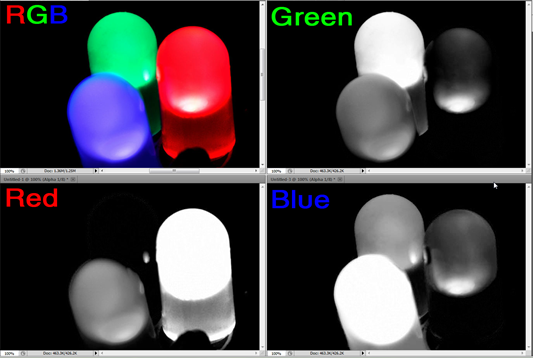
\includegraphics[width=\linewidth]{Bilder/RGB.png}
\setcaptioncitation{ https://www.howtogeek.com/wp-content/uploads/2011/02/sshot-74.png}
\caption{RGB Kanäle}
\label{fig: RGB}
\end{figure}
Abbildung \ref{fig: RGB} zeigt wie die einzelnen Kanäle arbeiten. Informationen aus dem Grundbild die Rot erscheinen, werden im roten Kanal besonders hell dargestellt. 
Ausschnitte aus der originalen Abbildung die blau erscheinen, werden im blauen Kanal ebenso heller dargestellt. Analog zu den beiden Beispielen arbeitet ebenso der grüne Kanal.
Werden die drei Kanäle wieder miteinander verbunden entsteht das Ausgangsbild. Der Vorteil solcher mehrkanaligen Formate ist, dass praktisch alle Informationen aus dem original Bild erhalten bleiben. Der Nachteil jedoch wird deutlich, wenn die Farbe für den Anwendungsfall keine oder eine geringe Rolle spielt. Da in dieser Arbeit Emotionen anhand von Gesichtern erkannt werden sollen, spielt die Farbe der Bilder selber eine untergeordnete Rolle, da diese keine nützlichen Informationen für das zu trainierende Modell enthält. Es wäre sogar kontraproduktiv. Dadurch dass mehr Kanäle mit Informationen vorhanden sind, muss auch das Modell mehr Daten bekommen, um zu lernen, wie die Informationen aus diesen zu verstehen sind. Dies wird auch von dem sogenannten ''Fluch der Dimensionalität'' beschrieben. Auf den Anwendungsfall bezogen bedeutet dies nur, dass je mehr Eigenschaften ausgewertet werden sollen, desto mehr Daten zum Lernen vorhanden sein müssen. Um dem präventiv entgegenzuwirken, ohne in Verlegenheit zu geraten, die Testdatensätze später erweitern zu müssen, können auch Bilder verwendet werden, die auf weniger Kanäle an Informationen zurückgreifen. Sogenannte Grayscale- oder Graustufenbilder bieten hier den Vorteil, dass es nicht drei, sondern lediglich einen Farbkanal gibt. In diesem wird ein Wert pro Pixel gespeichert. Je höher dieser Wert, desto weißer der Pixel, je niedriger, desto schwärzer. Dieses Format eignet sich bestens für das hier behandelte Modell, da keine wichtigen Informationen entfallen, die in einer farbigen Version des Bildes vorhanden währen, während sich aber die Anzahl der Daten verringert, die benötigt werden um das Modell erfolgreich trainieren zu können. Dies erhöht wiederum die Chance das zuvor definierte Should-Kriterium zu erfüllen, welches besagt, dass die Wahrscheinlichkeit zur Erkennung der richtigen Emotion über 50\% liegen muss. 
\chapter{Stand-Alone Lösung mit Schwerpunkt OpenCV}
\chapterauthor{2356667}
Während der weiteren Ausarbeitung des Konzeptes und der darauf basierenden Umsetzung sind letztendlich zwei verschiedene Lösungen entstanden. Aufgrund von Problemen, die innerhalb des Entwicklungsprozesses im Zusammenhang mit dem Hardwarekonzept aufgetreten sind, konnte das erste Projekt, so wie es geplant war, nicht zu Ende gebracht werden. Da dieser Ansatz jedoch als Grundlage für die letztendlich finale Lösung diente, werden sowohl das Konzept als auch die Umsetzung der ersten Lösung nachfolgend genauer erläutert.

\section{Konzept}
\sectionauthor{2356667}
Im Folgenden wird das in der Planungsphase entwickelte Konzept zur Emotionserkennung unter verschiedenen Aspekten, wie der Architektur und der Kommunikation, erläutert.

\subsection{Interaktionskonzept}
\sectionauthor{2356667}
Von außen betrachtet steht zuerst die Planung eines Interaktionskonzeptes an, in welcher Form der Nutzer die Möglichkeit hat, Input zur Verarbeitung zu liefern und an Output zu gelangen. Dem Anwender soll es möglich sein, schnell und verständlich mit dem Produkt zu interagieren, weshalb eine geeignete Benutzeroberfläche mit zwei wesentlichen Interaktionsoptionen erforderlich ist. Der aktuelle Video-Stream einer internen oder externen Kamera sollte als Input zur Emotionsanalyse verwendet werden und das Ergebnis der analysierten Sequenzen soll ausgegeben werden können. Um dies zu erreichen, soll die Bildbverarbeitungsbibliothek OpenCV verwendet werden, mit der sowohl der Zugriff auf alle verfügbaren Kameraeingabegeräte als auch die Darstellung von Bildern und Text in einer grafischen Benutzeroberfläche (GUI) in Form eines Fensters möglich ist. Die vom Nutzer gelieferten Videosequenzen sollen entsprechend bearbeitet werden, um anschließend eine Emotion zu erkennen und den entstandenen Output an die durch OpenCV generierte Oberfläche weiterzugeben. Der Output wird dem Nutzer letztendlich so dargestellt, dass dieser als einfache Textausgabe auf dem Bildschirm erscheint.\newline
Zusammenfassend kann man also sagen, dass der Nutzer aufgrund der Übersichtlichkeit lediglich mit der von OpenCV generierten Oberfläche interagieren kann und sich zu keinem Zeitpunkt mit den dahinterliegenden Komponenten der Emotionserkennung befassen muss.\newline

\subsection{Architektur}
\sectionauthor{2356667}

\subsubsection{Programmierumgebung}
\sectionauthor{2356667}
Aufgrund der Vorkenntnisse und Relevanz innerhalb des Studiums soll die Programmiersprache Python in aktuellster Version (3.6.9) vorrangig verwendet werden, jedoch kann unter gegebenen Umständen womöglich auch die Programmiersprache C++ eingesetzt werden, was noch zu prüfen ist. Auf eine bestimmte IDE wie PyCharm, Emacs oder Visual Studio Code wird sich an dieser Stelle nicht festgelegt, da dies jedem Entwickler selbst zu überlassen ist. Diesbezüglich sind nur Einschränkungen aufgrund der gewählten Rechnerarchitektur und der Programmiersprache zu berücksichtigen.\newline
Zur Entwicklung einer Emotionserkennung sollen als grundlegende Komponenten die Programmbibliothek OpenCV zur Bildverarbeitung und das Framework Tensorflow bzw. die Deep-Learning-Bibliothek Keras verwendet werden. Da das Einsatzgebiet von OpenCV in der Bildverarbeitung liegt, soll die Bibliothek dazu genutzt werden, den Input so zu verändern, dass dieser vom Modell zum Trainieren oder Vorhersagen einer oder mehrerer Emotionen verwendet werden kann. Für den wesentlichen Teil der Arbeit, das Entwickeln eines Modells, welches menschliche Emotionen anhand eines Bildausschnittes von einem Gesichts erkennen kann, ist die Deep-Learning-Bibliothek Keras zu verwenden.
\subsubsection{Hardware}
\sectionauthor{2356667}
Der Einfachheit halber wird zum Entwickeln als grundlegende Komponente ein handelsüblicher Laptop genutzt. Dabei wird außerdem auf das Open-Source Betriebssystem Ubuntu 18.04.4 LTS in der 64-bit Variante zurückgegriffen. Als zugrundeliegende Ressourcen stehen ein 8 Gigabyte großer Arbeitsspeicher sowie ein Intel Core i5-4210 Quadcore Prozessor mit einer Taktfrequenz von 4 x 2,60 GHz zur Verfügung. Des Weiteren kann die dedizierte Grafikkarte GeForce 820M mit einem Grafikkartenspeicher von 2046 MB verwendet werden. Der Festplattenspeicher von 500 GB kann im Umfang dieser Arbeit vernachlässigt werden, da es im Zusammenhang mit Gesichts- bzw. Emotionserkennung primär darauf ankommt, wie viel Rechenleistung zur Verfügung steht und nicht, wie groß die Speicherkapazität des Laufwerks ist. Um das rechenintensive Trainieren des Modells zur Emotionserkennung in akzeptabler Zeit zu garantieren, soll die Rechenleistung des Prozessors und der Grafikkarte vollständig genutzt werden können.

\section{Umsetzung}
\sectionauthor{2356667}
In diesem Kapitel wird die Umsetzung der auf dem entwickelten Konzept basierenden Lösung näher erläutert. Es handelt sich dabei um den Stand-Alone Laptop mit installiertem Ubuntu 18.04.4 LTS, wobei der Input und der Output auf OpenCV GUIs basiert.

\subsection{Input GUI}
\sectionauthor{2356667}
Als Einstieg in das Themengebiet Emotionserkennung bzw. Gesichtserkennung ergibt es Sinn, sich zuerst mit den Grundlagen der Bildverarbeitung und den Grundlagen von OpenCV vertraut zu machen. Aufgrund der aufgestellten Anforderungen ist es außerdem notwendig, eine grafische Oberfläche zu implementieren, mit der der Nutzer interagieren kann. Wie bereits in dem Konzept beschrieben, soll es dem User daher möglich sein, mithilfe der Webcam und einer grafischen Oberfläche, welche mit OpenCV programmiert wird, ein Bild als Input zu liefern. Wie man in Abbildung \ref{fig:Input GUI 1} sehen kann, wird im ersten Schritt die grafische Oberfläche erstellt und der Video Stream der Webcam in der Oberfläche angezeigt. Der zugehörige Codeausschnitt kann dem Anhang \ref{lst:Code Input GUI 1} entnommen werden.
\begin{figure}[h]
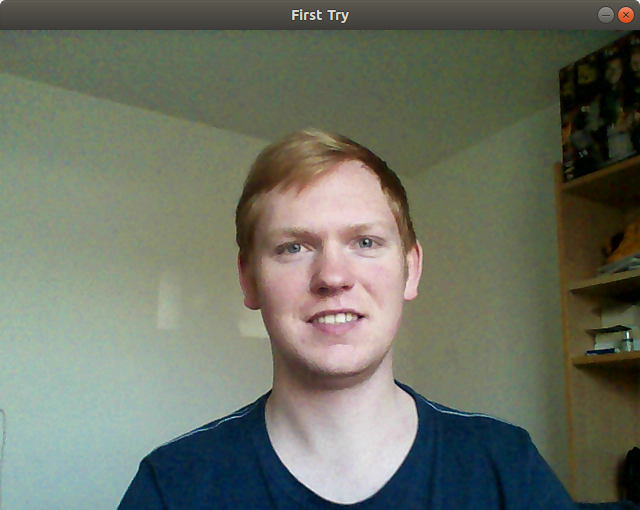
\includegraphics[width=\linewidth]{Bilder/InputGUI1.png}
\caption{GUI mit Video Stream der Webcam als Output}
\label{fig:Input GUI 1}
\end{figure}
Nachdem man nun auf den Video Stream der Webcam zugreifen und diesen wiedergeben kann, gilt es den relevanten Bildausschnitt, die sogenannte Region Of Interest (ROI), zu identifizieren. Da wir uns im Umfeld der Gesichts- und Emotionserkennung befinden, sind für uns alle Bereiche relevant, die ein menschliches Gesicht enthalten. Standardmäßig stellt OpenCV einige Modelle zur Objekterkennung zur Verfügung, welche problemlos genutzt werden können. Um so ein vortrainiertes OpenCV-Modell zur Gesichtserkennung einzubinden, kann man folgende Zeile an den Anfang des Codes schreiben:\newline
\lstinputlisting[style=custompython, numbers=none, linerange=3-3, caption=Einbinden eines vortrainierten OpenCV-Modells zur Gesichtserkennung]{Code/InputGUI2.py}
Mithilfe der Methode \texttt{detectMultiScale} des eingebundenen Modells, können nun die Koordinaten sowie die Höhe und die Breite von jedem in dem Bild gefundenen Gesicht extrahiert werden. Aufgrund dieser Informationen kann man den bisherigen Code nun so erweitern, dass ein Rechteck um jedes im Video Stream der Webcam gefundene Gesicht gezeichnet wird und über die grafische Oberfläche sichtbar gemacht wird. Das Resultat des entstandenen Codes \ref{lst:Code Input GUI 2} kann der Abbildung \ref{fig:Input GUI 2} entnommen werden.
\begin{figure}[h]
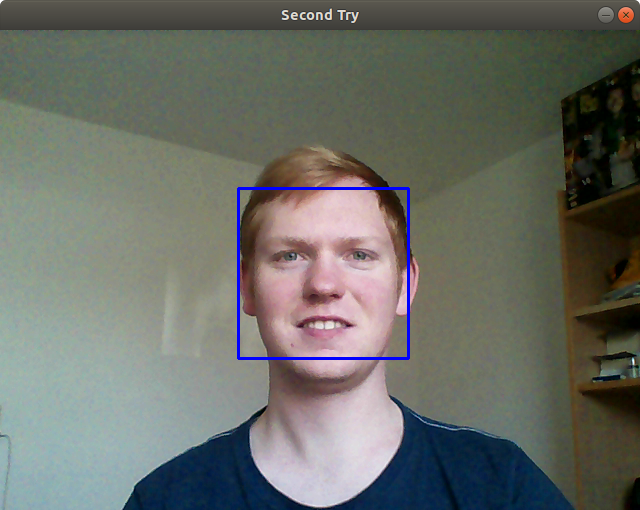
\includegraphics[width=\linewidth]{Bilder/InputGUI2.png}
\caption{GUI mit Video Stream der Webcam und markierten Gesichtern als Output}
\label{fig:Input GUI 2}
\end{figure}
Nun lässt sich noch darüber diskutieren, ob es weitere besonders zu berücksichtigende ROIs gibt. Im Zusammenhang mit Emotionen können unter anderem die Augen und der Mund eine besondere Rolle spielen, sodass nachfolgend beispielhaft das Hinzufügen eines Modells zur Erkennung der Augen in jedem bereits entdeckten Gesicht gezeigt wird. Dazu muss zusätzlich zum OpenCV-\texttt{CascadeClassifier haarcascade\_frontalface\_default.xml} der \texttt{CascadeClassifier haarcascade\_eye.xml} eingebunden werden. Um nun alle Augen in einem Bild zu erkennen, kann wieder die Methode \texttt{detectMultiScale} des Modells genutzt werden. Dem nachfolgenden Bildausschnitt \ref{fig:Input GUI 3} kann man nun entnehmen, wie um alle Augen, die sich in dem Bildausschnitt befinden in dem auch ein Gesicht erkannt wurde, ein grünes Rechteck gezeichnet wird.
\begin{figure}[h]
  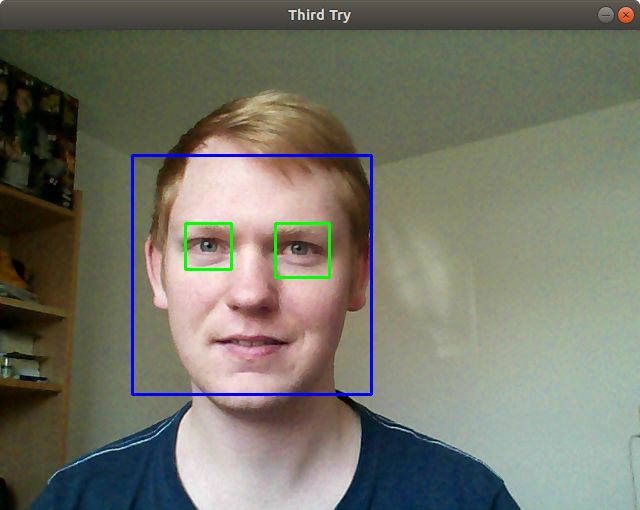
\includegraphics[width=\linewidth]{Bilder/InputGUI3.png}
  \caption{GUI mit Video Stream der Webcam und markierten Gesichtern und Augen als Output}
  \label{fig:Input GUI 3}
\end{figure}
Somit ist man nun in der Lage, alle relevanten Bereiche zu identifizieren und zu markieren. Um diese relevanten Regionen nun als Input für ein Modell zum Vorhersagen einer Emotion nutzen zu können, müssen die entsprechenden Bereiche jedoch ersteinmal abgespeichert werden. Um die Vergleichbarkeit der Bilder untereinander und die Vergleichbarkeit des zu testenden Bildes zu den trainierten Bildern zu gewährleisten, sollten diese vom gleichen Format sein. Wie bereits in der Theorie erwähnt, ist es außerdem sinnvoll entsprechende Ausschnitte nicht im Farbmodus abzuspeichern, sondern lediglich als Grayscale-Grafik. Die Erweiterung des bereits entstandenen Codes um die erleuterten Aspekte kann man am Code \ref{lst:Code Input GUI 3} sehen. Somit ist es dem Nutzer möglich, schnell und unkompliziert Bilder mit der Webcam zu machen und dort enthaltene Gesichter so zu speichern, dass sie als Input zum Vorhersagen einer Emotion genutzt werden können.

\subsection{Dataset}
\sectionauthor{2356667}
Zum Trainieren eines Modells zur Emotionserkennung wird das Cohn-Kanade Dataset zur Analyse von Emotionen verwendet.\footcite[Vgl.][]{CK} In dem verwendeten Dataset sind ca. 10000 Grayscale-Bilder enthalten, welche die in \ref{tab:ckemotions} zu sehenden Emotionen umfassen.
\begin{table}[h]
\centering
\begin{tabular}[t]{l|c}
Emotion & Anzahl nutzbarer Bilder \\
\hline
Anger & 45 \\
Contempt & 18 \\
Disgust & 59 \\
Fear & 25 \\
Happy & 69 \\
Sadness & 28 \\
Surprise & 83 \\
\hline
\end{tabular}
\caption{Emotionen mit jeweiliger Anzahl an Bildern}
\label{tab:ckemotions}
\end{table}
Es fällt auf, dass sich die dargestellte Anzahl von ca. 325 nutzbaren Bilder stark von der bereits erwähnten Anzahl von 10000 Bildern unterscheidet. Das liegt daran, dass das Dataset ursprünglich für die Analyse von Emotionensverläufen und nicht direkt für die Emotionserkennung an sich entwickelt wurde. Was das genau heißt, wird durch die Abbildung \ref{fig:Disgust} verdeutlicht.
\begin{figure}[h]
	\begin{minipage}[b]{.2\linewidth} % [b] => Ausrichtung an \caption
		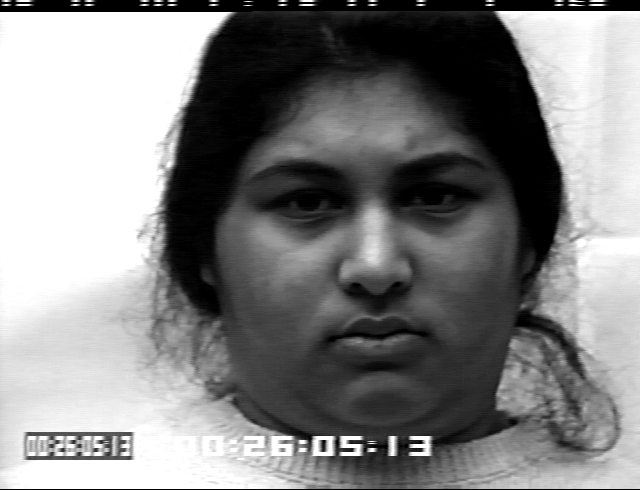
\includegraphics[width=\linewidth]{Bilder/Disgust1.png}
	\end{minipage}
	\hspace{.025\linewidth}% Abstand zwischen Bilder
	\begin{minipage}[b]{.2\linewidth} % [b] => Ausrichtung an \caption
		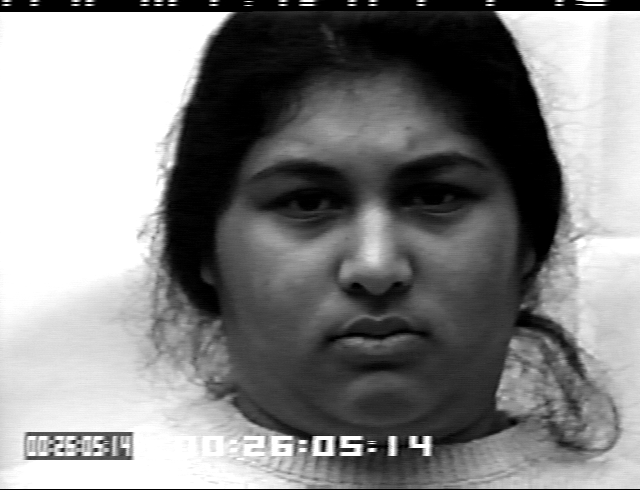
\includegraphics[width=\linewidth]{Bilder/Disgust2.png}
	\end{minipage}
	\hspace{.025\linewidth}% Abstand zwischen Bilder
	\begin{minipage}[b]{.2\linewidth} % [b] => Ausrichtung an \caption
		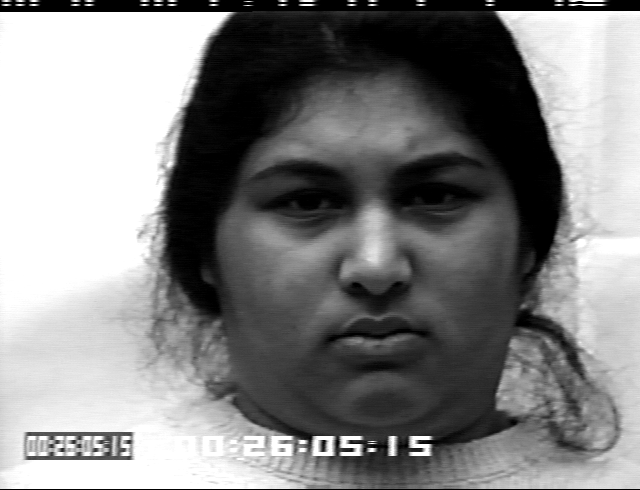
\includegraphics[width=\linewidth]{Bilder/Disgust3.png}
	\end{minipage}
	\hspace{.025\linewidth}% Abstand zwischen Bilder
	\begin{minipage}[b]{.2\linewidth} % [b] => Ausrichtung an \caption
		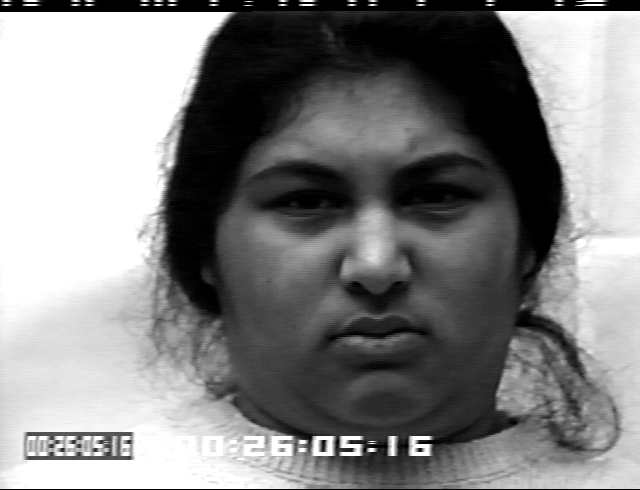
\includegraphics[width=\linewidth]{Bilder/Disgust4.png}
	\end{minipage}
	\newline
	\begin{minipage}[b]{.2\linewidth} % [b] => Ausrichtung an \caption
		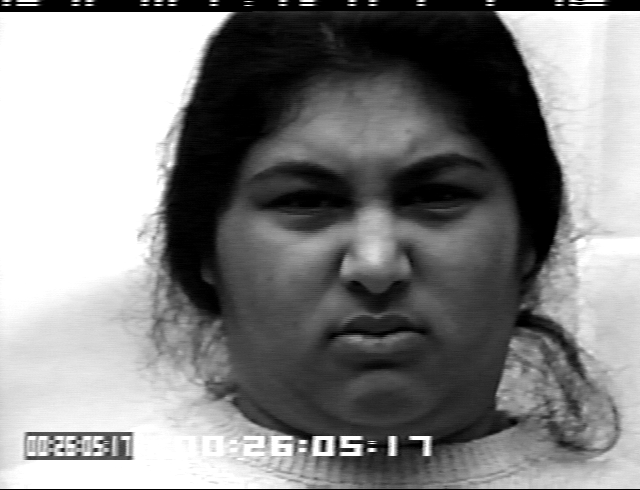
\includegraphics[width=\linewidth]{Bilder/Disgust5.png}
	\end{minipage}
	\hspace{.025\linewidth}% Abstand zwischen Bilder
	\begin{minipage}[b]{.2\linewidth} % [b] => Ausrichtung an \caption
		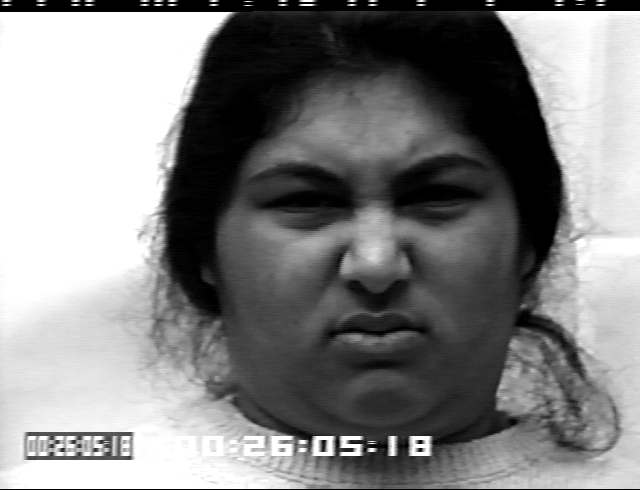
\includegraphics[width=\linewidth]{Bilder/Disgust6.png}
	\end{minipage}
	\hspace{.025\linewidth}% Abstand zwischen Bilder
	\begin{minipage}[b]{.2\linewidth} % [b] => Ausrichtung an \caption
		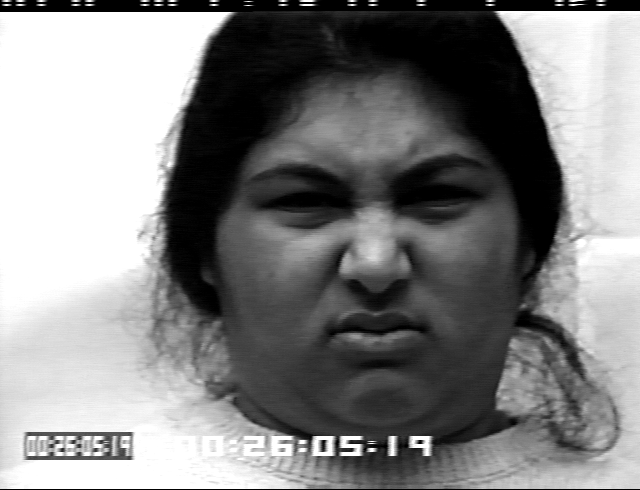
\includegraphics[width=\linewidth]{Bilder/Disgust7.png}
	\end{minipage}
	\hspace{.025\linewidth}% Abstand zwischen Bilder
	\begin{minipage}[b]{.2\linewidth} % [b] => Ausrichtung an \caption
		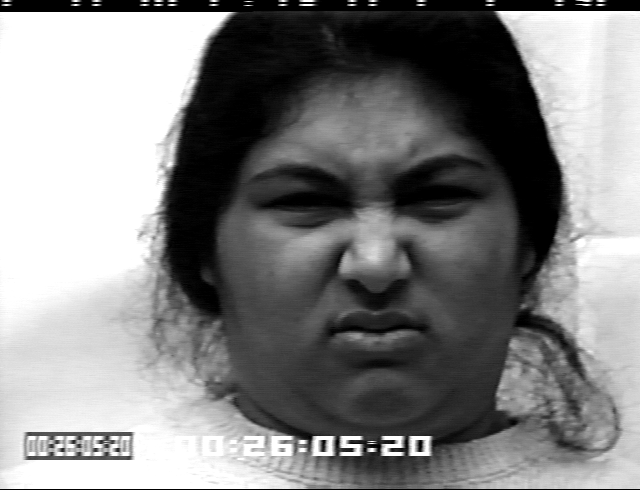
\includegraphics[width=\linewidth]{Bilder/Disgust8.png}
	\end{minipage} 
	\newline
	\begin{minipage}[b]{.2\linewidth} % [b] => Ausrichtung an \caption
		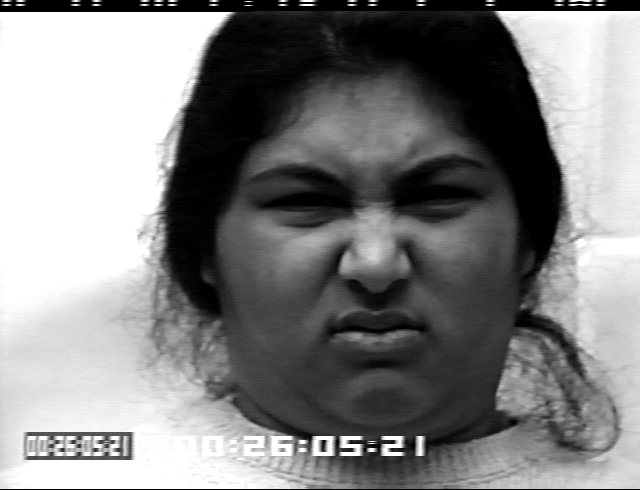
\includegraphics[width=\linewidth]{Bilder/Disgust9.png}
	\end{minipage}
	\hspace{.025\linewidth}% Abstand zwischen Bilder
	\begin{minipage}[b]{.2\linewidth} % [b] => Ausrichtung an \caption
		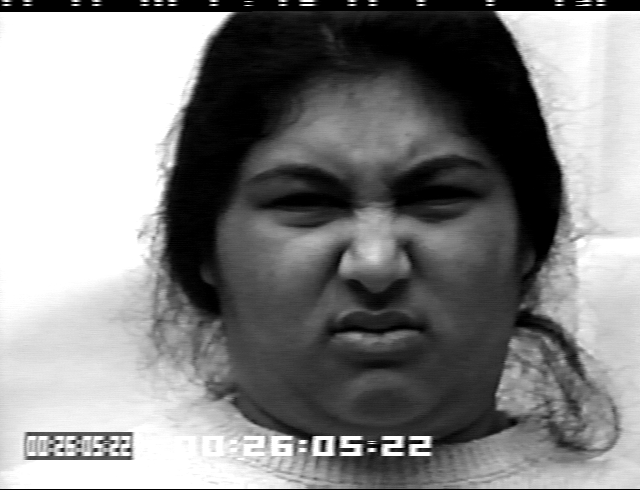
\includegraphics[width=\linewidth]{Bilder/Disgust10.png}
	\end{minipage}
	\hspace{.025\linewidth}% Abstand zwischen Bilder
	\begin{minipage}[b]{.2\linewidth} % [b] => Ausrichtung an \caption
		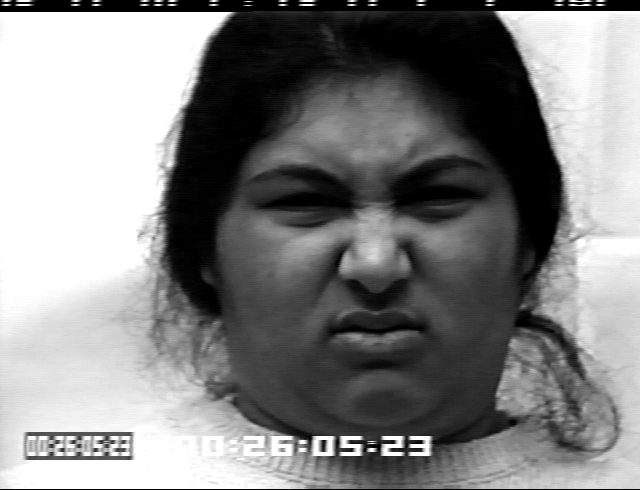
\includegraphics[width=\linewidth]{Bilder/Disgust11.png}
	\end{minipage}
	\caption{Emotionsverlauf von Neutral zu Disgust}
	\label{fig:Disgust}
\end{figure}

Jeder Datensatz beinhaltet mehrere Bilder, die den Verlauf einer Emotion von neutral bis hin zur jeweiligen Emotion darstellen. Da dieser Verlauf für die Emotionserkennung allenfalls für die Klassifizierung in Ausprägungen innerhalb einer einzelnen Emotion relevant wäre und somit im Umfang dieser Arbeit nicht betrachtet wird, wird nur das jeweils letzte Bild dieses Verlaufs, also die vollständig ausgeprägte Emotion, zum Trainieren des Modells genutzt. Somit ergibt sich der Unterschied von der Anzahl der jeweils letzten Bilder der Verläufe, ca. 325, und der Anzahl der Gesamtbilder aller Verläufe, ca. 10000.
Zur Verzeichnisstruktur des Datasets kann man sagen, dass es grundsätzlich zwei verschiedene Ordner gibt. In einem Ordner befinden sich alle Bilder, also die Verläufe der Emotionen und in dem anderen befinden sich mit der gleichen Struktur die dazugehörigen Emotionen in Textdateien. Die Darstellungen der beiden Strukturen als Verzeichnisbäume können der Anlage \ref{fig:Struktur CK Dataset} entnommen werden. Wie man den Verzeichnisbäumen entnehmen kann, ist die Struktur in beiden Ordnern identisch. In der ersten Ebene befinden sich Ordner jeweils mit 'S' aufgeteilt nach Personen. Innerhalb jeder dieser Personenordner gibt es einen oder mehrere weitere Ordner. Diese Ordner auf der 2. Ebene sind dreistellig aufsteigend numeriert und beinhalten jeweils einen Emotionsverlauf. Im Sachzusammenhang bedeutet dies, dass jede Person eine oder mehrere verschiedene Emotionsverläufe darstellt. Die Syntax der Dateinamen in den aufsteigend numerierten Ordner, die letztendlich den Emotionsverlauf beinhalten, ist \texttt{<Personenordner>\_<Emotionsverlaufsordner>\_<Pos. im Verlauf>.png} wobei die Position im Verlauf 8-stellig ist. Nimmt man die in Abbildung \ref{fig:Disgust} gezeigten Bilder als Grundlage, könnten die einzelnen Dateinamen wie im Verzeichnisbaum \ref{fig:Tree Emotionsverlauf} aussehen.
\begin{figure}
\dirtree{%
.1 images.
.2 S005\DTcomment{Person 1}.
.3 001\DTcomment{Emotionsverlauf 1}.
.4 S005\_001\_00000001.png.
.4 S005\_001\_00000002.png.
.4 S005\_001\_00000003.png.
.4 S005\_001\_00000004.png.
.4 S005\_001\_00000005.png.
.4 S005\_001\_00000006.png.
.4 S005\_001\_00000007.png.
.4 S005\_001\_00000008.png.
.4 S005\_001\_00000009.png.
.4 S005\_001\_00000010.png.
.4 S005\_001\_00000011.png.
.2 \ldots.
}
\caption{Struktur Emotionsverlauf}
\label{fig:Tree Emotionsverlauf}
\end{figure}
Aus der dargestellten Struktur des Ordners, in dem sich sämtliche Bilder befinden und den jeweiligen Dateinamen lassen sich keinerlei Rückschlüsse auf die dargestellten Emotionen ziehen. Um herauszufinden, welche Emotion durch welchen Emotionsverlauf dargestellt wird, muss man in das entsprechende Verzeichnis innerhalb des Ordners mit den gelabelten Emotionen schauen. Dort befindet sich dann eine Textdatei, die den selben Dateinamen hat, wie das letzte Bild aus dem dazugehörigen Emotionsverlauf. In dieser Datei befindet sich dann eine Fließkommazahl, die für die jeweilige Emotion in Tabelle \ref{tab:ckemotions} steht. Um nun herauszufinden, welche Emotion durch den in Abbildung \ref{fig:Tree Emotionsverlauf} gezeigten Emotionsverlauf dargestellt wird, schaut man in das Verzeichnis \texttt{emotions/S005/001/}, in dem sich die Datei \texttt{S005\_001\_00000011.txt} befindet. In dieser Datei würde dann \texttt{3.0000000e+00} stehen, was sich gemäß der Tabelle mit \texttt{Disgust} gleichsetzen lässt.\newline
Um später ein vernüftiges superviesed Learning auf Grundlage des Datasets durchführen zu können, wird eine eigene Verzeichnisstruktur erstellt, die sortiert nach Emotionen jedes letzte Bild eines Emotionsverlaufs beinhaltet. Zusätzlich wird die Emotion neutral hinzugefügt, da jedes erste Bild eines Emotionsverlaufs als neutrale Ausgangslage dient. Der entwickelte Algorithmus zum Überarbeiten und Sortieren des Datasets und die daraus resultierende neue Verzeichnisstruktur können dem Code \ref{lst:Organising The Dataset} und der Abbildung \ref{fig:Tree Sorted Set} im Anhang entnommen werden.

\subsection{Training}
\sectionauthor{2356667}
Zum Trainieren eines Modells stellt OpenCV verschiedene Klassifizierer zur Verfügung, jedoch wird sich in diesem Abschnitt immer auf das Supervised Learning des FisherFaceRecognizer bezogen, welcher mit dem im vorherigen Schritt präparierten Dataset trainiert wird. Da das Dataset schon sortiert und vorbereitet wurde, ist es nun sehr leicht, eine Methode zu schreiben, die ein Array mit Trainingsdaten und ein Array mit den zugehörigen Labels liefert. Aufgrund der Verzeichnisstruktur des Datasets kann man über alle Emotionsordner iterieren, dabei alle Grayscale-Bilder in das Array mit den Trainingsdaten einlesen und die jeweilige Emotion in das Array mit den Labeln einlesen. Dabei ist jedoch zu beachten, dass die Labels bzw. die Emotionen als Integer-Werte beginnend mit 0 und aufsteigend dargestellt werden müssen. Das heißt, die Ordnernamen, welche den Emotionen als Text entsprechen, müssen in Integer-Werte konvertiert werden, indem man z.B. den jeweiligen Index der Emotion in dem globalen Emotions-Array \ref{lst:Emotions-Array} nimmt.
\lstinputlisting[style=custompython, numbers=none, linerange=5-5, caption=Emotions-Array, label=lst:Emotions-Array]{Code/ClassifierHandler.py}
Die vollständige Methode zum Extrahieren der Trainigsdaten ist im Anhang unter \ref{lst:Trainingsdaten extrahieren} gelistet. 
Da nun die erforderlichen Arrays mit Trainingsdaten und Labeln erzeugt werden können, beschäftigt man sich als nächstes mit dem zu trainierenden Klassifizierer, dem sogenannten FisherFaceRecognizer. Die \texttt{FisherFaceRecognizer}-Klasse stellt die statische Methode \texttt{create()} und die Methode \texttt{train(InputArray data, InputArray labels)} zur Verfügung welche im Code \ref{lst:Classifier Handler} zum Trainieren benutzt werden. Es fällt somit deutlich auf, dass die Komplexität des eigentlichen Trainierens im Vergleich zur Vorbereitung des Datasets wesentlich geringer ist.

\subsection{Testing}
\sectionauthor{2356667}
Das Testen des im vorherigen Schritt trainierten Modells kann aufgrund der Vorarbeit ebenfalls mit sehr geringem Zeitaufwand implementiert werden. Aufgrund der, wie sich später herausstellte, sehr geringen Datengrundlage und der Should-Anforderung gemäß MoSCoW Priorisierung, dass die Wahrscheinlichkeit zur Erkennung der richtigen Emotion über 50\% liegen soll, wird anstatt der üblichen Aufteilung des Datasets in Trainings- und Testdaten das komplette Dataset als Trainingsdaten genutzt. Daraus ergibt sich dann, dass ein anderes Verfahren zum Testen des Klassifiziers gefunden werden muss. Somit wird zum Testen des Modells eine grafische Oberfläche erstellt, die im speziellen als Echtzeitanalyse der Emotionen fungiert. Hierzu kann ein Großteil des Codes genutzt werden, der als Vorarbeit bei der Entwicklung der Input GUI implementiert wurde. Der Ablauf eines konkreten Tests ist dann das Starten der Oberfläche, welche den Video Stream der Webcam ausgibt und gleichzeitig jedes Einzelbild vom Modell analysieren lässt. Dies geschieht, wie ebenfalls bereits beschrieben, durch das Ausschneiden des Gesichtes und das anschließende Konvertieren in das Grayscale-Format sowie daraufhin das Vorhersagen einer Emotion. Das Gesicht wird dann mit einem Rechteck markiert und darüber wird die vorhergesagte Emotion ausgegeben. Verändert man den Code der Input GUI nur geringfügig und erweitert ihn um das Vorhersagen der Emotion und das Schreiben der vorhergesagten Emotion auf den Output Video Stream, dann erhält man den im Anhang \ref{lst:Text mit Input GUI} gezeigten Code.

\subsection{Optimierung der Lösung}
\sectionauthor{2356667}
Durch das Testen des Modells konnte festgestellt werden, dass trotz der vergrößerten Menge an Daten zum Trainieren die Genauigkeit der Vorhersagen mit ca. 20\% deutlich unter den in den Anforderungen definierten 50\% liegt. Aufgrund dieser Tatsache wird versucht, den Trainingsprozess zu optimieren. Die Möglichkeiten zum komplexen Konfigurieren eines Modells in OpenCV sind begrenzt, sodass eine Konfiguration, die wesentlich mehr Features der Emotion als zuvor analysiert, erschwert wird. Außerdem würde sich dann die Tatsache bemerkbar machen, dass OpenCV keine Möglichkeit bietet, die  Rechenleistungen der CPU und der GPU zu kombinieren. Daraus würde sich ein sehr langwieriger Trainingsprozess ergeben, was nicht mehr den definierten Anforderungen entsprechen würde. Daher wird zunächst versucht, den Prozess in eine extra dafür vorgesehene Bibiliothek auszulagern, wobei die Entscheidung auf die Keras-API gefallen ist. Keras selbst dient in unserem Fall als Schnittstelle zum Tensorflow-Framework. Auf die genaue Funktionsweise von Keras wird in einem späteren Kapitel näher eingegangen. An dieser Stelle bleibt nur noch zu bemerken, dass die Installation von Keras und das Einbinden benötigter Komponenten zwar erfolgreich durchgeführt werden konnten, jedoch die Ausführen der benötigten Komponenten aufgrund einer nicht unterstützten Prozessorarchitektur bzw. eines nicht unterstützten Chipsets nicht möglich war. Aufgrund der benötigten Ressourcen und der mit Tensorflow kompatiblen Architektur wurde sich deshalb für eine Server-Client-Architektur entschieden.

\chapter{Server-Client Lösung}
\chapterauthor{2356667}
Basierend auf den Erfahrungen, die während des Entwicklunsprozesses der Stand-Alone Lösung gewonnen werden konnten, werden das Konzept und dementsprechend auch die Umsetzung überarbeitet und optimiert. Nachfolgend wird die damit finale Lösung genauer erläutert.

\section{Konzept}
\sectionauthor{2356667}
Die Interaktionsmöglichkeiten, die der Nutzer haben soll, bleiben unverändert. Der Übersichtlichkeit halber soll ausschließliche mit einer mithilfe von OpenCV generierten grafischen Oberfläche interagiert werden. Die wesentlichen Änderungen beschränken sich auf die Systemarchitektur, insbesondere auf die Programmierumgebung.

\subsection{Programmierumgebung}
Zusätzlich zu den bereits erwähnten Gründen für die Entscheidung der Programmiersprache Python ist noch die Wiederverwendbarkeit der bisher entwickelten Lösung zu nennen. Um den Anforderungen bezüglich der dem Projekt zur Verfügung stehenden Zeit gerecht zu werden, wird weiterhin die Programmiersprache Python verwendet, da so der bisher implementierte Code als Grundlage dienen kann und die neue Lösung darauf aufbauend entwickelt werden kann. Außerdem stellt sich nun die Frage, mit welcher Entwicklungsumgebung gearbeitet wird. Da nun auf einer Cloud-Infrastruktur entwickelt wird, sind die reinen grafischen Umgebungen wie Visual Studio Code oder PyCharm nicht zu empfehlen. Aufgrund vieler Vorteile, die dem entsprechenden Kapitel zu entnehmen sind und der ebenfalls bereits erwähnten Relevanz innerhalb des Studiums, wird zum weiteren Entwickeln die Open-Source Webapplikation Jupyter Notebook verwendet. Da über das Webinterface insbesondere das Debugging vereinfacht wird, kann vor allem der Entwicklungsprozess signifikant beschleunigt werden. Der Einheitlichkeit halber wird die Clientanwendung ebenfalls mithilfe von Jupyter Notebook entwickelt, wobei diese in der finalen Version durch minimale Anpassungen auch problemlos ohne Jupyter Notebook ausführbar gemacht werden kann. OpenCV, die Programmbibliothek für Bildverarbeitung und Keras, die Deep-Learning-Bibliothek, werden weiterhin für die bereits beschriebenen Zwecke verwendet.

\subsection{Hardware}
\sectionauthor{2356667}
Der Server wird in Cloudumgebung gehostet, die Infrastructure as a Service (IaaS) für Wissenschaft und Bildung bereitstellt. Hier ist besonders hervorzuheben, dass durch die Cloudumgebung eine hohe Flexibilität bezüglich der Skalierbarkeit gewährleistet ist. Hinsichtlich der verfügbaren Ressourcen wird ein Paket gewählt, das 4 virtuelle CPUs sowie 16 Gigabyte Hauptspeicher beinhaltet. Sollte im Verlauf der Umsetzung auffallen, dass die standardmäßig zur Verfügung gestellten Ressourcen nicht ausreichen, können diese bis zu 16 vCPUs und bis zu 32 Gigabyte RAM erweitert werden. Die vordefinierte Größe der Festplatte von 12 GB sollte für den Umfang des Projektes ausreichen, jedoch kann auch hier die Kapazität um bis zu 50 Gibibytes erhöht werden. Weiterhin wird auf das Betriebssystem Ubuntu 18.04 gesetzt, da so ein Großteil der zuvor gewonnen Erfahrung genutzt werden kann.

\section{Umsetzung}
\sectionauthor{2356667}
Trotz der aufgetretenen Komplikationen bei der Entwicklung einer Stand-Alone Lösung muss an dieser Stelle erwähnt werden, dass große Teile, gerade im Bereich des Inputs und Outputs wiederverwendet werden. Die auf Grundlage der Stand-Alone Version entwickelte Server-Client Lösung wird nachfolgend genauer erläutert.

\subsection{Dataset}
\sectionauthor{2356667}
Im Zuge der vertieften Recherche zu Keras und der direkten Verwendung im Bereich Gesichts- und Emotionserkennung konnte ein besseres Dataset als zuvor gefunden werden. Das Dataset gehört zu einer Open-Source Facial Expression Recognition auf der Plattform Kaggle.\footcite[Vgl.][]{FER-Challenge} Kaggle ist eine Online-Community deren Hauptzweck es ist, Data-Science-Wettbewerbe auszuschreiben, an denen jeder interessierte teilnehmen kann. Außerdem wird durch die Plattform ermöglicht, Datensätze zu finden und zu veröffentlichen und ggf. Modelle auszuprobieren oder ebenfalls zu veröffentlichen. Vereinfacht kann mann sagen, dass Kaggle ein virtueller Treffpunkt für Data-Scientists in den Bereichen maschinelles Lernen und KI-Entwicklung ist.\newline
Nun wird das im Projekt verwendete Dataset betrachtet. Das Dataset umfasst 35887 Datensätze, die allesamt gelabelt sind. Dabei wird das Set in Trainingsdaten, Public-Testdaten und Private-Testdaten unterteilt, wobei 80\% aller Werte auf das Trainingsset entfallen und jeweils 10\% auf die beiden Testsets. Die Unterteilung der Testdaten in Public und Private ist dabei nur im direkten Zusammenhang mit dem Kaggle-Wettbewert von Relevanz, da ein Set zum Testen des Modells für die Entwickler selbst vorgesehen ist und das Andere, um einen Sieger der Challenge auszumachen. Da wir mit unserem Modell nicht an der Facial Emotion Recognition Challenge teilnehmen, kann man die beiden Testsets zu einem großen zusammenfassen. Damit erhält man 28709 Datensätze zum Trainieren des Modells und 7178 Datensätze zum Testen. Aufgrund der Menge an Daten werden diese nicht wie beim anderen Dataset in einer Ordnerstruktur mit entsprechend vielen Bilddateien zur Verfügung gestellt, sondern als Comma-Separated-Values in einer CSV-Datei. Dabei handelt es sich um eine Art Tabelle, deren Struktur der nachfolgenden Tabelle \ref{tab:FER2013} zu entnehmen ist.
\begin{table}[h]
\centering
\begin{tabular}[t]{c|l|c}
emotion & pixels & Usage \\
\hline
0 & 70 80 82 72 58 58 60 63 54 58 60 48 89 115 121 119 115 110 98 ... & Training \\
0 & 151 150 147 155 148 133 111 140 170 174 182 154 153 164 173 178 ... & Training \\
2 & 231 212 156 164 174 138 161 173 182 200 106 38 39 74 138 161 ... & Training \\
4 & 24 32 36 30 32 23 19 20 30 41 21 22 32 34 21 19 43 52 13 26 40 ... & Training \\
6 & 4 0 0 0 0 0 0 0 0 0 0 0 3 15 23 28 48 50 58 84 115 127 137 142 ... & Training \\
2 & 55 55 55 55 55 54 60 68 54 85 151 163 170 179 181 185 188 188 ... & Training \\
4 & 20 17 19 21 25 38 42 42 46 54 56 62 63 66 82 108 118 130 139 ... & Training \\
3 & 77 78 79 79 78 75 60 55 47 48 58 73 77 79 57 50 37 44 56 70 80 ... & Training \\
0 & 254 254 254 254 254 249 255 160 2 58 53 70 77 76 75 78 68 18 32 ... & PublicTest \\
0 & 170 118 101 88 88 75 78 82 66 74 68 59 63 64 65 90 89 73 80 80 ... & PrivateTest \\
\hline
\end{tabular}
\caption{Struktur des CSV-Datasets der FER-Challenge}
\label{tab:FER2013}
\end{table}
Die Spalte \texttt{emotion} kann dabei Werte von 0 bis 6 annehmen, wobei sich insgesamt 7 verschiedene Werte ergeben, die den Emotionen entsprechend der Tabelle \ref{tab:feremotions} zugeordnet werden können. Außerdem werden in der Tabelle die absoluten und relativen Häufigkeiten der Emotionswerte dargestellt, da diese für spätere Optimierungen relevant sind.
\begin{table}[h]
\centering
\begin{tabular}[t]{c|c|c|c}
Wert & Emotion & $H_n$ & $h_n$ \\
\hline
0 & Angry & 4953 & 13,80\% \\
1 & Disgust & 547 & 1,52\% \\
2 & Fear & 5121 & 14,27\% \\
3 & Happy & 8989 & 25,05\% \\
4 & Sad & 6077 & 16,93\% \\
5 & Surprise & 4002 & 11,15\% \\
6 & Neutral & 6198 & 17,27\% \\
\hline
\end{tabular}
\caption{Zuordnung und Häufigkeiten der Emotionen}
\label{tab:feremotions}
\end{table}
Die Grafik \ref{fig:visualisierungferemotions} stellt eine visualisierte Häufigkeitsverteilung der angegebenen absoluten Häufigkeiten dar.
\begin{figure}[H]
  \centering
\begin{tikzpicture}
	\begin{axis}[
	  ybar,
	  axis x line = bottom,
	  enlarge x limits = .1,
	  bar width=20pt,
	  nodes near coords,
	  symbolic x coords ={Angry, Disgust, Fear, Happy, Sad, Surprise, Neutral},
	  x tick label style={rotate=45,anchor=north east}%,
	  %title = {Häufigkeitsverteilung der Emotionen}
	  ]
	  \addplot[fill=blue] coordinates {
		(Angry,4953)
		(Disgust,547)
		(Fear,5121)
		(Happy,8989)
		(Sad,6077)
		(Surprise,4002)
		(Neutral,6198)
	  };
	\end{axis}
  \end{tikzpicture}
  \caption{Häufigkeitsverteilung der Emotionen}
  \label{fig:visualisierungferemotions}
\end{figure}
Nun werden die anderen Spalten betrachtet. In der Spalte \texttt{pixels} befinden sich die eigentlichen Bilddaten als Pixelwerte, die lediglich mit einem Leerzeichen getrennt in einem String dargestellt werden. In Tabelle \ref{tab:FER2013} wird nur ein kleiner Ausschnitt der insgesamt 2304 Pixelwerte pro Datensatz angezeigt. Aus der Darstellung der Bilder im Grayscale-Format ergeben sich die in der Theorie bereits erläuterten Pixelwerte von 0 bis 255. Die Anzahl von 2304 Pixeln ergibt sich durch die Länge und die Breite der Bilder von jeweils 48 Pixel mal 48 Pixel. Bevor man die Bilddaten in Form des Strings aus Pixeln für das Modell nutzen kann, müssen diese erst entsprechend formatiert und umgeformt werden, aber dazu später mehr. Die letzte der Tabelle zu entnehmende Information befindet sich in der Spalte \texttt{Usage}. Dort wird jedem Datensatz zugeordnet, ob er im Zuge des Wettbewerbes zum Trainieren, zum privaten Testen oder zum öffentlichen Testen verwendet wird.

\subsection{Modell}
\sectionauthor{1329241}
Nachfolgend wird das für die Emotionserkennung erstellte Modell mit den jeweils einzelnen Layern näher erläutert. Die komplette Struktur des Modells kann der Abbildung \ref{fig:Model Summary} im Anhang entnommen werden.
Wie zu sehen ist, ist das Modell ein einfaches konvolutionales neuronales Netzwerk. 
Wie der Grafik zu entnehmen ist sind die Eingabedaten 48 x 48 Pixel große Bilder, die wiederum durch drei sequentielle Schichten von Convolutional Layern und Pooling Layern verarbeitet werden. Jede dieser drei Schichten weist dabei wiederum drei Conv2D-Layer auf. Diese sind in Keras Convolutional-Layer. Jeder von diesen hat dabei 32 Filter als Verarbeitungsparameter, die wiederum eine Größe von 3 x 3 Pixeln aufweisen. Die Aktivierungsfunktion jedes dieser Conv2D-Layer ist die Relu Funktion, die bereits in Kapitel \ref{Aktivierungsfunktion} erläutert wurde. Die Padding-Strategie für diese Schichten ist ''same''. Das bedeutet, dass die Bilder über die die Filter der Conv2D-Layer laufen am Rand so aufgefüllt werden, dass die resultierenden Ausgabedaten ebenfalls 48 x 48 Pixel groß sind, und sich nicht nach jedem  Convolutional-Layer verkleinern. Auf die jeweils drei Conv2D-Layer folgt ein Pooling Layer. Dieser verwendet die Max. Pooling Strategie und hat eine Größe von 2 x 2 Pixeln. Dadurch halbieren sich die Größen der Eingabebilder jeweils von 48 x 48 Pixeln auf 24 x 24 bzw. 12 x 12 und 6 x 6. Der Anschließende Flatten-Layer formatiert die 6 x 6 Bilder und die jeweiligen 32 Filter um, sodass die darauffolgenden Dense-Layer (Vollständig verbundene Layer) die Bilder verarbeiten können. Die drei Dense-Layer Verdichten die Ausgabeneuronen so, dass am Ende für jede Emotion die vorhergesagt werden kann ein Neuron als Ausgabeknoten übrig ist. Aktivierungsfunktionen der ersten beiden der drei Dense-Layer ist die Relu Funktion. Die Letzte Schicht hingegen verwendet für die Ausgabe die Softmax Funktion, diese ermöglicht es die Wahrscheinlichkeiten für die jeweilige Emotion auszugeben.

\subsection{Trainieren des Modells}
\sectionauthor{2356667}
Sobald das beschriebene Modell kreiert wurde, kann mit dem wesentlichen Teil, dem Trainieren, fortgefahren werden. Ein definiertes Modell besitzt in Keras die Methode \texttt{fit}, deren Verwendung im einfachsten Fall folgendermaßen aussieht: \texttt{fit(x=Trainingsdaten, y=Trainingslabels)}, wobei \texttt{x} und \texttt{y} in diesem Fall Numpy-Arrays sind. Die Trainingsdaten und die entsprechenden Labels erhält man aus dem Dataset, jedoch müssen diese noch in das erforderliche Format, eine Matrix bzw. ein Numpy-Array konvertiert werden. Dazu müssen die bereits erwähnten Pixel in der Zeichenkette in eine Matrix der Form 48 Pixel x 48 Pixel gebracht werden, wobei wiederum jedes Pixel als eindimensionales Array mit einem Element dargestellt wird. Sollten an dieser Stelle Farbbilder mit dem Format 48 Pixel x 48 Pixel als Input genutzt werden, hätte man anstatt der Struktur \texttt{(48, 48, 1)} entsprechend der drei RGB-Werte Daten der Struktur \texttt{(48, 48, 3)}. Optional können der Methode \texttt{fit} Validierungsdaten und die zugehörigen Labels als Tupel übergeben werden. Dabei ist zu beachten, dass beide Komponenten als Numpy-Array vorliegen müssen und es analog zu den Trainingsdaten einer Konvertierung in das passende Format bedarf. Der Methode \texttt{fit} zum Trainieren des Modells können außerdem einige optionale Parameter mitgegeben werden, die im Zusammenhang mit den Validierungsdaten besonders für die Optimierung des Modells, dem Hyperparameter-Tuning, wichtig sind.\newline
Als Rückgabewert liefert die angesprochene Methode ein History-Objekt, in welchem Daten wie Loss und Accuracy der Trainingsdaten und ggf. Loss und Accuracy der Validierungsdaten während des Trainingsprozesses aufgezeichnet wurden. Das History-Objekt existiert jedoch nur innerhalb der Laufzeit des Python-Skripts und wird nicht zusammen mit dem Modell über die API-Methode \texttt{save(path="modelToSave.model")} abgespeichert. Um die History eines Modells jederzeit anzeigen, ausgeben und ggf. visualisieren zu können, werden die aufgezeichneten Daten zusätzlich zum Modell im JSON-Format abespeichert und können bei Bedarf über entprechende Bibliotheken wieder geladen und in ein Dictionary konvertiert werden.\newline
Die Visualisierungen der aufgezeichneten Daten inklusive entsprechender Testdaten mithilfe der Bibliothek \texttt{matplotlib} können der Abbildung \ref{fig:Visualize History} im Anhang entnommen werden.
\begin{figure}[H]
	\begin{minipage}[b]{\linewidth}
		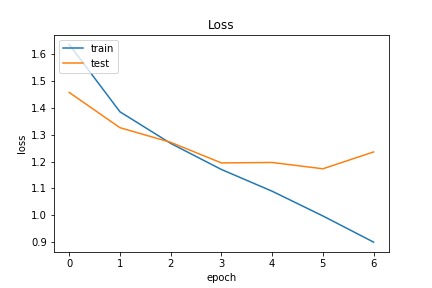
\includegraphics[width=\linewidth]{Bilder/loss_history.png}
	\end{minipage}
	\begin{minipage}[b]{\linewidth}
		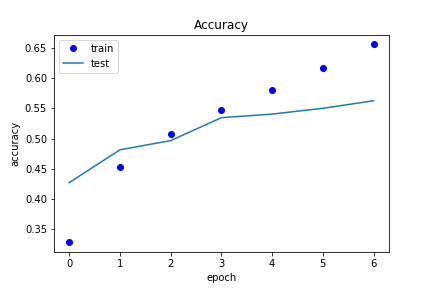
\includegraphics[width=\linewidth]{Bilder/accuracy_history.png}
	\end{minipage}
	\caption{Visualisierung der aufgezeichneten Daten des History-Objektes}
	\label{fig:Visualize History}
\end{figure}

\subsection{Testen des Modells}
\sectionauthor{2356667}
Beim Testen des Modells benötigt man analog zum Trainieren eines Modells mehrere Datensätze und deren jeweilige Label. Um eine Genauigkeit zu ermitteln, lässt man sich die Label des Testsets vom trainierten Modell vorhersagen und gleicht diese mit den tatsächlichen Labeln ab. Voraussetzung dafür ist, dass die Testdaten dem selben Format wie die Trainingsdaten, also einer \texttt{(48, 48, 1)}-Matrix, entsprechen. Mithilfe der Keras API-Methode \texttt{predict}, der man die gesamten Trainingsdaten auf einmal übergeben kann, kann man sich auf Grundlage des Modells die Labels vorhersagen lassen. Die konkrete Rückgabe der Methode ist ein Array, dessen Anzahl der Elemente der Anzahl an Trainingsdaten entspricht. Dabei ist wiederum jedes Element selbst ein Array, dessen Länge der Anzahl an möglichen Emotionen entspricht. Übergibt man beispielsweise 10 Testdatensätze und das Modell wurde mit 4 Emotionen trainiert, erhält man ein zweidimensionales Array, welches 10 Arrays der Länge 4 enthält. In den inneren Feldern sind für jede Emotion Werte zwischen 0 und 1 enthalten. Da diese einer Art Wahrscheinlichkteit entsprechen, ergeben sie kumuliert den Wert 1. Vereinfacht gesagt wird für jede Emotion, die als Input gegeben wird, die prozentuale Übereinstimmung mit jeder möglichen Emotion zurückgegeben bzw. die Wahrscheinlichkeit zu jeder möglichen Emotion vorhergesagt. Dies könnte beispielhaft so aussehen: \texttt{[0.05690899, 0.09713534, 0.5027235,  0.04000191, 0.29613075, 0.00709949]}. Möchte man zu einem Input eine einzige Emotion vorhersagen, ist es sinnvoll, die dem Maximum des Arrays entsprechende Emotion zurückzugeben. Nimmt man die in Tabelle \ref{tab:feremotions} definierte Zuordnung von Emotionen als Grundlage, entspricht das Maximum des Arrays dem Index 2, wobei dieser Wert wiederum der Emotion \texttt{Fear} zugeordnet ist.\newline
Gleicht man die vorhergesagten Emotionen mit den tatsächlichen Emotionen ab, kann man eine statistische Auswertung über der Gesamtmenge aller Daten vornehmen, z.B. dass die Wahrscheinlichkeit einer richtigen Vorhersage bei 40\% liegt. Außerdem ist es möglich, den Anteil der richtigen Zuordnung jeder einzelnen Emotion, z.B. \texttt{[0.1, 0.2, 0.05, 0.15, 0.91, 0.34]} zu ermitteln. Dem letzteren Beispiel kann man entnehmen, dass das Modell sehr gut geeignet ist, die Emotion, die dem Wert 4 entspricht, zu erkennen, jedoch sehr schlecht darin ist, alle anderen Emotionen zu erkennen. Beide Daten werden während des Testprozesses berechnet und sind bei der späteren Optimierung des Modells hilfreich.

\subsection{Optimierung des Modells}
\sectionauthor{1329241}
Um das Modell nun zu optimieren wurden einige Schritte unternommen. Zum einem wurde die Layer-Anordnung und auch Anzahl im Laufe der Arbeit verändert. Dabei konnten mit der vorliegenden Anordnung die aus der Grafik \ref{fig:Model Summary} zu entnehmen ist, die besten Ergebnisse erzielt werden. Die Konfiguration der einzelnen Layer wurde ebenfalls überarbeitet, vor allem hinsichtlich der Aktivierungsfunktion, Optimierungsfunktion, der Verlustfunktion, aber auch der allgemeinen Verarbeitungsparameter wie Padding-Strategie oder Filtergröße und Anzahl. Es wurden ebenso Optimierungen an der Epochen-Anzahl und Batch size vorgenommen. Letztlich wurden insgesamt 7 Epochen - Also sieben ganze Durchläufe zum Trainieren des Modells - vorgenommen, die jeweils eine Batch size von  64 aufweisen. Da zum Trainieren 80\% des Gesamtdatensatzes verwendet wurden, also insgesamt $ 28709 $ Bilder, werden pro Epoche insgesamt $ 448 $ Durchläufe mit 64 Bildern, und ein Durchlauf mit $ 37 $ Bildern durchgeführt. Diese Anzahl kommt dadurch zu Stande, dass bei mehr Epochen ein Overfitting an den Trainingsdaten zu erkennen war. Die Batch size hingegen wurde so gewählt, um das Modell schnell und gleichzeitig weniger Ressourcen-intensiv zu gestalten. Die Optimierung des Modells generell folgt ein wenig dem trial and error Prinzip. Es gibt zwar einige Empfehlungen 
\footcite[Vgl.][]{ModellOptimierung}
 - vor allem hinsichtlich der Hyperparameter wie Epochengröße und Batch size - jedoch gibt es keine generell beste Lösung die auf alle Anwendungsfälle passt. Deshalb müssen die besten Einstellungen für Hyperparameter zu dem jeweiligen Datensatz und Modellaufbau ''gefunden'' werden

\subsection{Webserver}
\sectionauthor{2356667}
Einer der wesentlichen Unterschiede zu der zuvor entwickelten Lösung ist die Architektur. Es läuft nicht mehr alles lokal auf einem Rechner, sondern es wird zwischen Server und Client unterschieden. Alles was das Modell direkt betrifft, also das Trainieren, Testen und Vorhersagen, geschieht auf dem Server, wo auch das Modell selbst existiert. Um mit dem Client interagieren zu können, wird das Webframework Flask verwendet, welches konkret als Webserver dient. Da Flask in Python geschrieben ist, wird die Implementierung von Endpunkten in Verbindung mit den bereits implementierten Funktionalitäten sehr stark vereinfacht.\newline
Die Interaktion zwischen Server und Client ist sehr überschaubar und es wird lediglich ein einziger Endpunkt auf der Serverseite benötigt. Dieser Endpunkt nimmt mittels der \texttt{POST}-Methode ein vom Client geliefertes, grob vorbearbeitetes Bild entgegen. Dieses Bild wird dann auf dem Server so formatiert, dass mithilfe eines bereits trainierten Modells eine Emotionsvorhersage getroffen werden kann. Das Ergebnis wird dann an den Client zurückgeliefert und kann dort in einen entsprechenden Kontext, wie die reine Ausgabe oder die Analyse eines Pokerfaces, gesetzt und weiterverwendet werden.\newline
Damit der Server mithilfe eines Modells Vohersagen machen und Bilder archivieren kann, werden zur Initialisierung das Modell geladen und entsprechende Ordnerstrukturen angelegt, sofern diese noch nicht vorhanden sind. Danach kann der Webserver gestartet werden, um Verbindungen vom Client über einen vordefinierten Port entgegenzunehmen. Sobald ein Client ein Bild an den Server übergibt, wird dieses gespeichert bzw. archiviert. Da nicht sichergestellt ist, dass der Client ausschließlich Bilder der Größe 48 Pixel x 48 Pixel mit einem Gesichtsausschnitt  sendet, werden diese zunächst serverseitig geprüft und ggf. überarbeitet werden.  
Die allgemeine Vorgehensweise ist dabei, zuerst ein Gesicht zu erkennen und dieses danach auf 48 Pixel x 48 Pixel zuzuschneiden. Damit das Modell eine optimale Vorhersage geben kann, wird der Ausschnitt des extrahierten Gesichtes ggf. noch in ein Graustufenformat konvertiert. Um nun einen validen Input für das Modell zu generieren, wird das Image-Objekt in einen Pixel-String bzw. in eine Matrixrepräsentation der Form \texttt{(48, 48, 1)} gebracht. Jetzt kann auf dem bei der Initialisierung geladenen Modell die bereits erläuterte Methode \texttt{predict} aufgerufen werden. Der Rückgabewert dieser Funktion bzw. die Vorhersagewerte der einzelnen Emotionen werden dann an den Client zurückgegeben.

\subsection{Client}
\sectionauthor{2356667}
Der Hauptzweck der Client-Anwendung ist die Darstellung des Output mithilfe einer grafischen Benutzerschnittstelle. Im Hintergrund interagiert der Client mit dem Server, indem er Webcam-Bilder liefert, die hinsichtlich der Emotion auf dem Server analysiert werden und erhält Vorhersage-Matrizen. Die Interpretation dieser Werte obliegt dem Client, der diese dem Nutzer auf bestimmte Weise zugänglich macht. Die Anwendung umfasst somit zwei wesentliche Funktionalitäten, eine grafische Oberfläche zur Interaktion mit dem Anwender und im Hintergrund die Netzwerkkommunikation mit dem Server. Da nach den definierten Anforderungen keine komplexen Interaktionen mit dem Nutzer notwendig sind, umfasst die GUI lediglich ein Fenster in dem der Video-Stream der Webcam ausgegeben wird. Zusätzlichen enthält das Fenster, als Schriftzug in einer Ecke des Bildes, die Information, ob es sich laut Definition um ein Pokerface handelt oder nicht. Somit kann der Nutzer seine aktuelle Emotion sehen und die Ausgabe, ob ein Pokerface vorhanden ist oder nicht, besser nachvollziehen. Da die Ausgabe des Video-Streams im Fenster und die Netzwerkkommunikation grundsätzlich voneinander unabhängig sind, können diese Aufgaben in zwei verschiedene Prozesse bzw. Threads aufgeteilt werden. Wird dies nicht gemacht, kann es je nach Auslastung des Netzwerkes oder Ressourcenknappheit auf der Serverseite zu einer ruckeligen und verzögerten Ausgabe des Video-Stream kommen. Somit werden im Hauptprozess die grafischen Aufgaben, wie die Ausgabe des Video Streams und des Schriftzuges, erledigt und in einem zweiten Thread wird die Kalkulation des Pokerfaces und der Informationsaustausch mit dem Server geregelt. Um Daten zwischen den beiden Threads auszutauschen werden globale Variablen genutzt. Die Information, ob es sich um ein Pokerface handelt oder nicht, wird z.B. vom sekundären Thread in eine globale Variable geschrieben und vom GUI-Thread ausgelesen. In definierten Intervallen kann der Thread, der unter anderem mit dem Server kommuniziert, einzelne Bilder des Video-Streams abgreifen und zur Vorhersage an den Server schicken, ohne dass bei der grafischen Ausgabe auf die Antwort des Servers gewartet werden muss. Wie bereits erwähnt, werden die vom Server gelieferten Daten clientseitig interpretiert, was konkret bedeutet, dass ein Algorithmus implementiert werden muss, der anhand der Vorhersagedaten entscheidet, ob ein Pokerface vorhanden ist oder nicht. Um diese Auswertung eines Pokerfaces umzusetzen wurden zwei verschiedene Algorithmen entwickelt, welche im Folgenden genauer expliziert werden.

\subsubsection{Langzeit-orientierter Algorithmus}
\sectionauthor{8774695}
Die erste Umsetzung der clientseitigen Auswertung betrachtete das Szenario, einen Pokerspieler während der gesamten Dauer eines Poker-Spieles zu analysieren und in Echtzeit dem Anwender mitzuteilen, wenn der Gesichtsausdruck des Spielers von seinem üblichen Pokerface abweicht. In der Theorie sollte demnach ein leichtes Lächeln oder ein trauriger Gesichtsausdruck direkt erkannt werden und somit dem Anwender ein Feedback über das derzeitige Blatt des betrachteten Spielers geben.
Die Grundidee bei der Umsetzung des Algorithmus war es den Programmablauf in zwei Phasen einzuteilen. In der ersten Phase, der  \textit{\textbf{Initialisierungsphase}}, sollten Daten gesammelt und analysiert werden, um eine erste Vorstellung des Pokerfaces der zu betrachtenden Person zu bekommen. Um dies zu erreichen wird eine gewisse Anzahl an Bildern aufgenommen und die enthaltenen Emotionen validiert. Sollten die Bilder nahezu die selben Emotionen zeigen, könnte man davon ausgehen das diese das Pokerface der Person repräsentieren. Sollten die Bilder allerdings nicht ähnlich zueinander sein, also verschieden Emotionen zeigen, wird die Initialisierungsphase wiederholt, solange bis der Datensatz an aufgenommenen Bildern genügend Ähnlichkeiten aufweist. Sobald die Daten genügend Aufschluss über ein mögliches Pokerface generiert haben, geht das Programm in die  \textit{\textbf{Hauptphase}} über. Hier wird anhand der gewonnen Daten erkannt, ob ein Pokerface vorliegt oder die Person Emotionen zeigt. Die genaue Umsetzung des Algorithmus kann dem Programmablaufplan in Grafik \ref{fig:flowchart} entnommen werden, welcher im Folgenden erläutert wird.

%Unbedingt Grafik richtig Formatieren an der richtigen Stelle!!
\begin{figure}[H]
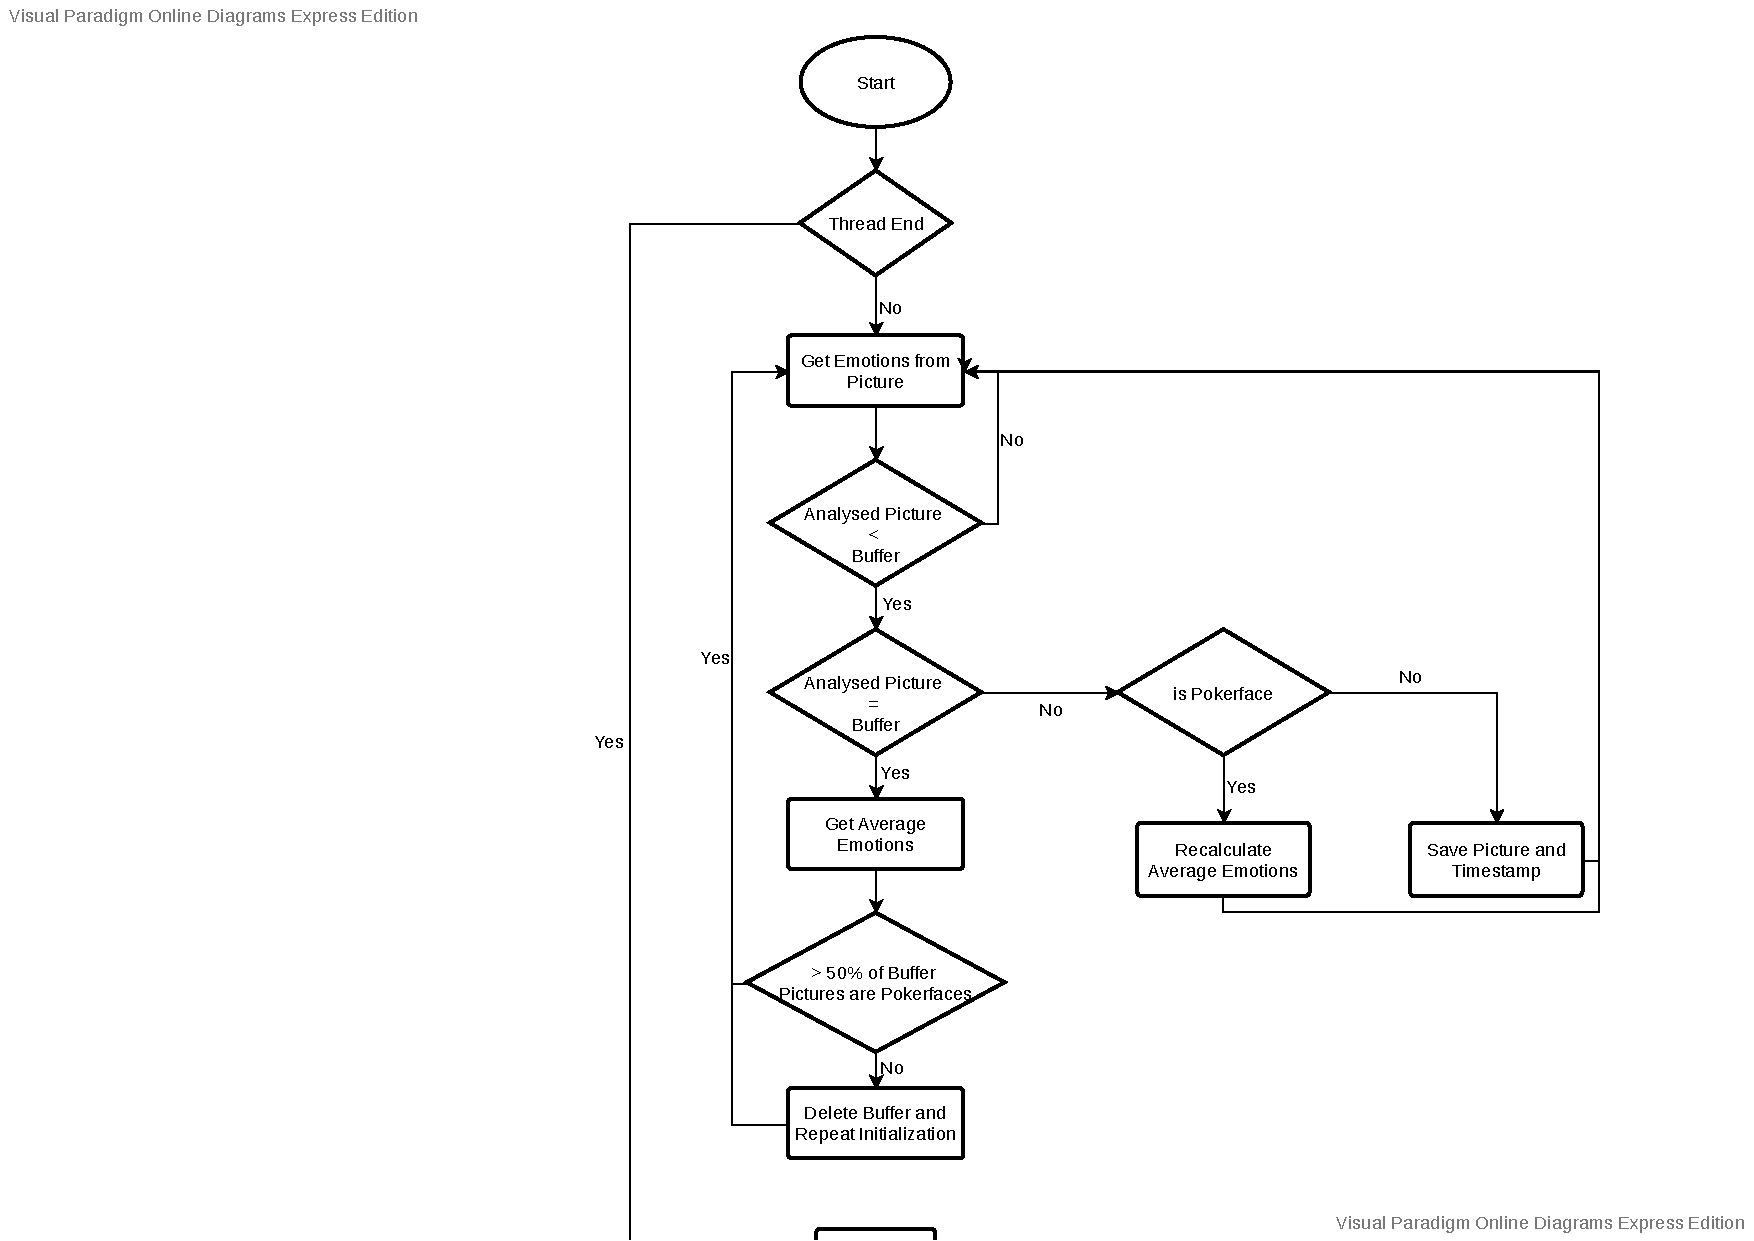
\includegraphics[width=\linewidth]{Bilder/ClientDataflow.pdf}
\caption{Programmablaufplan des Client-Programms}
\label{fig:flowchart}
\end{figure}

Der dargestellte Ablauf wird solange durchgeführt, bis der entsprechende Thread beendet wird. Zu Beginn wird ein Bild aufgenommen und über die Verbindung zum Server analysiert. Während der Initialisierungsphase wird dieser Vorgang wiederholt bis ein definierter Buffer gefüllt wurde. Dieser kann beispielsweise mit zehn Plätzen definiert worden sein, demnach zehn Bilder der Person aufgenommen werden und die ausgewerteten Emotionen aller Bilder im Buffer abgespeichert werden. Eine Formalere Formulierung wäre die Buffer Größe der Länge $ n $  , wobei $ n \in N $, welche die aggregierten Ergebnisse der Server-Evaluierung speichert. Jeder Eintrag innerhalb des Buffers ist wiederum eine Liste, welche die Emotionsvorhersagen beinhaltet. Eine mögliche Struktur eines Buffers der Länge zwei könnte wie folgt aussehen: $ \qquad[ [0.61, 0.30, 0.15, 0.01, 0.76, 0.95] , [0.31, 0.22, 0.51, 0.41, 0.01, 0.55] ] $
Sobald der Buffer mit den Emotionswerten gefüllt wurde, wird die Initialisierungsphase eingeläutet. Hier wird zuerst die durchschnittliche Emotionswahrscheinlichkeit aller Emotionen über die gespeicherten Werte berechnet. Am Beispiel der zuletzt genannten Liste würde für die Emotion \textit{Angry}, welche durch die erste Stelle der Liste repräsentiert wird, der Durchschnitt der Werte \textbf{0.61} und \textbf{0.31} berechnet werden. Diese Rechnung wird für jede Emotion durchgeführt. 
\newline
Um mit Gewissheit sagen zu können, dass man einen guten Durchschnitt aller Emotionen erhalten hat, welche ein Pokerface repräsentieren, sollten die zugrunde liegenden Daten auch möglichst Ähnlich sein. Werden beispielsweise bei zehn aufgenommenen Bildern verschiedene Grimassen geschnitten, wodurch die Bilder mal ein glückliches Bild und mal ein trauriges Bild zeigen, kann man annehmen, dass der Durchschnitt der Bilder nicht das Pokerface der Person darstellt. Demnach wird geprüft ob mindestens 50\% der Bilder innerhalb eines Toleranzbereichs des berechneten Durchschnitts liegen. Bei zehn Bildern sollten also fünf der Bilder möglichst gleiche Emotionen zeigen, wobei die anderen fünf Bilder natürlich keine starken Abweichungen darstellen dürfen.
Sollte dies nicht gelingen, kann man keine klare Aussage über das Pokerface der Person treffen und die Initialisierungsphase wird durch das Löschen des Buffers wiederholt.
Sollten allerdings die gewünschten Ergebnisse erzielt werden, kann mit den Durchschnittsemotionen ein Fazit über das Vorhandensein eines Pokerfaces getroffen werden und die Hauptphase wird eingeläutet. Hier werden die Analyseergebnisse der Bilder anhand der Durchschnittswerte und einem definierten Toleranzbereich verglichen und als Pokerface oder Nicht-Pokerface eingeordnet. Sollte das Bild als Pokerface eingeordnet werden, werden die Emotionen in die Durchnittsemotionen mit einberechnet. Dadurch kann die Genauigkeit der Emotionswerte des Pokerfaces während des Spiels gesteigert werden. Sollte das Bild außerhalb des Toleranzbereichs liegen, wird der Zeitpunkt und das dazugehörige Bild gespeichert und der Anwender wird über das Vorliegen eines Nicht-Pokerfaces informiert.
\newline
Der beschriebene Algorithmus ist in der Theorie eine gute Umsetzung für das Erkennen eines Pokerfaces während eines Pokerspiel, allerdings sehr fehleranfällig in der Praxis. Das Problem liegt in der Bewegung der zu betrachtenden Person. Sollte die Person beispielsweise Reden, verändert sich der Gesichtsausdruck und somit auch die Emotionswerte, wodurch sich der Algorithmus für ein Nicht-Pokerface entscheidet. Auch wenn die Person sich zurück lehnt oder in eine andere Richtung blickt, werden, selbst wenn sich der Gesichtsausdruck nicht verändert, neue Werte durch das Modell berechnet und die Ergebnisse unbrauchbar. Im schlechtesten anzunehmenden Szenario würde die Person sich nach einer erfolgreichen Initialisierung zurück lehnen und somit könnte man über den gesamten Spielverlauf keine Aussagen mehr über ein Pokerface treffen. 
Zudem liegt ein weitere Problem in der Annahme, dass die ausgerechneten Emotionswerte auch tatsächlich das Pokerface des Spielers repräsentieren. In der Praxis wäre es wohl eher unüblich den Gegenspieler zu bitten während der Initialisierungsphase sein Pokerface aufzusetzen. Bei einer Bufferlänge von 10 Bildern und einer Abtastrate des Streams von 0.2 Sekunden würde die Initialisierungsphase 2 Sekunden dauern. Gerade zum Beginn eines Spieles werden sich die Spieler noch miteinander unterhalten und nicht direkt ihr Pokerface aufsetzen. Aus diesem Grund ist es wahrscheinlicher, dass man ein 2 Sekunden dauerndes Lächeln des Spielers als Pokerface aufgreift und das wird kaum der Wahrheit entsprechen.
Aus diesen Gründen wurde sich für den zweiten Algorithmus entschieden, welcher im Folgendem vorgestellt wird.

\subsubsection{Kurzzeit-orientierter Algorithmus}
\sectionauthor{1329241}
Im Gegensatz zu dem letzten Algorithmus analysiert dieser die Kurzaufnahmen und nicht das gesamte Spiel. 
Wie in dem ersten Algorithmus wird auch hier der Videostream in einer gewissen Rate abgetastet. Diese Momentaufnahmen aus dem Videostream werden ebenfalls dem Server zum Evaluieren gegeben. Dieser Vorgang wird einige Male wiederholt, und die daraus resultierenden Daten aggregiert und zwischengespeichert. Das Ergebnis dieser Aggregation ist dann eine Liste der Länge 
$ n $  , wobei $ n \in N $
. Jedes Element dieser Liste ist wiederum eine Liste, die die Emotionsvorhersagen für ein bestimmtes Bild aus dem Videostream beinhaltet. So könnte z.B. eine solche Liste der Länge 2 folgende Struktur aufweisen: \newline
$ \qquad[ [0.61, 0.30, 0.15, 0.01, 0.76, 0.95] , [0.31, 0.22, 0.51, 0.41, 0.01, 0.55] ] $
Wobei jeweils ein Wert für eine Emotion steht bzw. die Wahrscheinlichkeit einer Emotion für das jeweilige Bild. Anhand dieser Liste wird dann wiederum die Abweichung der Emotionen in den Bildern festgelegt. Dazu werden die einzelnen Emotionswerte zuerst extrahiert und zusammengefasst - also alle fröhlichen, ängstlichen, neutralen, etc. Danach werden dann die Unterschiede in den jeweiligen Werten ermittelt.
Dies geschieht, indem zuerst der Mittelwert einer Emotion ermittelt wird, und dann die Werte gegen diesen geprüft werden. Weicht dabei eine Emotionsvorhersage zu weit von dem Mittelwert ab, wird zurückgegeben, dass ein Pokerface nicht vorliegen kann. Dies entspricht der Definition eines Pokerfaces in \ref{pokerface}, da dann je nach Toleranzwert der  wegen Messungenauigkeiten des Models eingeplant werden muss, eine zu hohe Abweichung einer Emotion in den Bildern gemessen wurde, und demnach der Gesichtsausdruck nicht beibehalten wurde.
Formal beschrieben wertet der Algorithmus also folgende Formel aus: \newline \newline
$ Eingabe $  sei eine Liste der Länge $ 6 $, wobei jedes Element dieser Liste wiederum eine Liste ist. Ein Element dieser Unterliste heißt dabei
 $ Emotion_{e} $, wobei $ e \in {\textit{1 \dots 6 }} $. $Emotion_{e}$ ist eine Liste der Länge $ n $ ist mit den Vorhersage Daten einer einzelnen Emotion wie z.B. \textit{fear} aus der Eingabeliste. $Emotion_{e}$ hat die Form $$ Emotion_{e} = \qquad [value_{1}, \dots ,value_{n}] $$ 
und 
$$average_{e} =\frac{1}{n} \cdot \sum_{i = 1}^{n} value_{i} $$
ist der Durchschnitt von $ Emotion_{e} $.
Für diese Werte gilt:
\newline $$ \forall value_{i} \in Emotion_{e} : (average_{e} - value_{i}) \leq \epsilon \Rightarrow Pokerface = True $$
 $ \epsilon$ ist hierbei die Toleranz in der sich eine Abweichung der Emotion begeben darf.


\chapter{Ergebnis}
\chapterauthor{2356667}
Nachfolgend werden die aufgrund des erstellten Konzeptes entwickelten Lösungsansätze und Lösungen erläutert. Dazu werden die definierten Anforderungen vor allem auch im Bezug auf das trainierte Modell zum Klassifizieren von den vordefinierten Emotionen und das Verifizieren und Testen dieses Modells auf Erfüllung geprüft.\newline
Eine grundlegende Anforderung ist, dass die Emotionen nicht zufällig erkannt werden. Hier kann gesagt werden, dass diese Anforderung schon in frühen Projektphasen erfüllt werden konnte und die Genauigkeit der richtigen Zuordnung der Testdaten bei 55,71\% liegt. Somit ist davon auszugehen, dass vorhandene Emotionen im Durchschnitt auf ca. jedem zweiten Bild richtig klassifiziert werden. Dies kann in der Praxis anhand von eigenen Tests nur so bestätigt werden. Ergänzt man die Tabelle \ref{tab:feremotions} der Häufigkeitsverteilung der Emotionen mit der Genauigkeit der Zuordnung der Testdaten zu den einzelnen Emotionen ergibt sich folgende Tabelle \ref{tab:genauigkeitemotions}.
\begin{table}[H]
  \centering
  \begin{tabular}[H]{c|c|c|c|c}
  Wert & Emotion & $H_n$ & $h_n$ & Genauigkeit \\
  \hline
  0 & Angry & 4953 & 13,80\% & 46,76\% \\
  1 & Disgust & 547 & 1,52\% & --------- \\
  2 & Fear & 5121 & 14,27\% & 33,4\% \\
  3 & Happy & 8989 & 25,05\% & 80,83\% \\
  4 & Sad & 6077 & 16,93\% & 39,45\% \\
  5 & Surprise & 4002 & 11,15\% & 73,65\% \\
  6 & Neutral & 6198 & 17,27\% & 49,39\% \\
  \hline
  \end{tabular}
  \caption{Genauigkeit der Zuordnung der Testdaten zu den einzelnen Emotionen}
  \label{tab:genauigkeitemotions}
\end{table} 
Bei Betrachtung der zwei Ansätze zur Erkennung eines Pokerfaces ist festzustellen, dass bei der Implementierung der Clientanwendung sowohl der langzeitorientierte als auch der kurzzeitorientierte Algorithmus zwischen Pokerface und kein Pokerface unterscheiden kann. Durch ausführliche Praxistests kann die grundsätzliche Funktionstüchtigkei für beide Algorithmen validiert werden. Die letzte Must-Anforderung ist die Implementierung einer benutzerfreundlichen Interaktionsmöglichkeit, um Input zu liefern und Output darzustellen. Dabei stellt der im Projektumfang definierte Output lediglich die Information dar, ob ein Pokerface vorhanden ist oder nicht. Die erste Teilanforderung wurde schon in den ersten Entwürfen erfüllt, da ohne besondere Interaktion des Anwenders die Bilder der Webcam bzw. des Video-Streams automatisiert als Input genutzt wurden. Die am Anfang erstellte OpenCV-Anwendung dient auch als Grundlage für die finale Version, weshalb die Teilanforderung dort ebenfalls erfüllt ist. Durch die einfache Textausgabe auf dem gespiegelten Video-Stream in der Clientanwendung, ob ein Pokerface vorhanden ist oder nicht, wird auch die zweite Teilanforderung, dass ein Output darzustellen ist, erfüllt.\newline
Dadurch dass die Genauigkeit zur Erkennung der richtigen Emotion bei über 50\% liegt, gilt auch die erste Anforderung der Should-Klassifizierung als erfüllt. Die genannte Genauigkeit ergibt sich aus den in Tabelle \ref{tab:genauigkeitemotions} dargestellten Daten. Hierbei ist zu bemerken, dass aufgrund der signifikant geringen Anzahl an Daten zu der Emotion \texttt{Disgust} entschieden wurde, im Umfang des Projektes lediglich die restlichen sechs Emotionen zu berücksichtigen. Somit wird zwischen mehr als fünf verschiedenen Emotionen differenziert und auch die zweite Anforderung der Should-Kriterien kann als erfüllt angesehen werden. Wie ebenfalls in den Anforderungen definiert, soll die Erkennung einer Emotion und eines Pokerfaces innerhalb eines Pokerspielzuges eines Spielers, also innerhalb von 20 Sekunden erfolgen. Nach ausgiebigen Praxistests der Clientanwendung kommt man zu dem Ergebnis, dass die Bilder bei einer guten Netzwerkverbindung zum Server in nahezu Echtzeit analysiert und die Ergebnisse an den Client zurückgesendet werden. Für zuverlässige Aussagen bezüglich des Pokerfaces müssen in beiden Algorithmen Referenzwerte gesammelt werden. Je nach Konfiguration der Anzahl der Referenzwerte und der Zeitdifferenz zwischen den Referenzwerten, vergehen bis zum ersten Erkennen eines Pokerfaces zwischen ca. fünf und zehn Sekunden. Beide Algorithmen laufen direkt auf dem Client und die Analyse der Emotionen erfolgt nahezu in Echtzeit, deshalb liegt die Dauer der Erkennung eines Pokerfaces nach Programmstart bei ca. 11 Sekunden und die reine Dauer zur Erkennung eines Pokerfaces liegt bei unter einer Sekunde. Somit gilt auch die letzte Should-Anforderung als erfüllt.\newline
Wie bereits mehrfach erwähnt, werden Bilder in nahezu Echtzeit analysiert, sodass die erste Anforderung nach der Could-Klassifikation ebenfalls als erfüllt gilt. Eine weitere Anforderung in dieser Kategorie ist das Trainieren des Modells innerhalb eines Arbeitstages. Bei den ersten Modellen, welche auf dem Dataset der FER-Challenge über 50 bis 100 Epochen trainiert wurden, lag die Trainingsdauer mit ca. 14 Stunden deutlich über einem Arbeitstag. Bei der Optimierung des Modells und dem Feintuning der Hyperparameter Batchsize und Epochs konnte die Genauigkeit des Modells erheblich gesteigert werden, wobei sich als Nebeneffekt die Trainingsdauer auf ca. 30 Minuten signifikant verbessert hat. Somit wurde mit der Optimierung des Modells auch indirekt die zuvor angesprochene Anforderung erfüllt. Da einzelne Bilder des Video-Streams der Webcam als Input zur Analyse dienen und diese automatisiert an den Server übermittelt werden sowie auch der Output mit der Information, ob ein Pokerface vorhanden ist oder nicht, automatisiert in der GUI ausgegeben wird, sind von Seiten des Nutzers keinerlei Interaktionen erforderlich. Dieser muss lediglich die Anwendung, also das Jupyter Notebook bzw. das Python-Skript ausführen. Dem Nutzer werden zur Interaktion keine Auswahlmöglichkeiten gegeben, weshalb für die reine Bedienung der Oberfläche kein technisches Wissen benötigt wird, jedoch sollte zum Starten des Skriptes ein geringes technisches Verständnis vorhanden sein. Aufgrund der MoSCoW-Klassifizierung dieser Anforderung als Could, kann diese nur zu einem Großteil erfüllt werden, was jedoch aufgrund der Klassifizierung kein Problem darstellt.\newline
Das Ziel des Projektes ist nicht die Analyse von ganzen Videos. Da immer einzelne Emotionen auf einzelnen Bildern analysiert werden, kann man hier zwar von der eingeschränkten Erfüllung der Anforderung sprechen, jedoch ist es nicht möglich, direkt ein Video zu analysieren. So wie bei der Anforderung, dass das Modell bei jeder Belichtung valide Ergebnisse liefern soll, handelt es sich um Anforderungen der Won't-Klassifizierung. Daher stellt es kein Problem dar, dass zur Analyse von Emotionen auf Bildern zumindest eine mäßige Belichtung notwendig ist, wobei für zuverlässige Ergebnisse verschiedene Belichtungseinstellung getestet werden sollten.

\let\cleardoublepage\relax
\chapter{Diskussion}
\chapterauthor{8774695}
In dem letzten Kapitel dieser Arbeit werden die Ergebnisse, das Vorgehen und die verwendete Literatur in diesem Projekt  kritisch betrachtet und reflektiert. Zuletzt sollen dem Leser noch einige Ideen vorgestellt werden, in welche Richtung die entwickelte Lösung in Zukunft möglicherweise weiterentwickelt werden kann und welche Änderungen und Verbesserungen dafür notwendig wären. Ziel dieses Kapitels ist es dem Leser die positiven und negativen Aspekte des Projektablaufs aufzuzeigen und in letzterem Fall welche Hürden diese beeinflusst haben. Hierdurch sollen dem Leser Anregungen gegeben werden, auf welche Einflussfaktoren bei künftig gleichartigen Projekten im Bereich der Gesichts- / Emotionserkennung zu achten sind.
Doch bevor die kritische Betrachtung im folgendem Vorgenommen wird, werden noch einmal kurz die Rahmenbedingungen des Projektes genannt. Das Projektteam besteht aus drei Studenten im sechsten Semester, welche vor dem Start des Projektes kaum nennenswerte Vorkenntnisse im Bereich von neuronalen Nezwerken und der Programmiersprache Python hatten. Für die Lösung der Aufgabenstellung standen insgesamt 32 Wochen zur Verfügung, welche innerhalb der Studien- und Arbeitszeit statt fand.

\section{Reflexion der Ergebnisse}
\sectionauthor{8774695}

Wie in dem letzten Kapitel zu sehen ist, wurden die definierten Anforderungen erfolgreich Umgesetzt. Die Bewertung der Anforderungen selbst wird in dem folgendem Kapitel genauer diskutiert. Nachdem der Erfolg des Projektes größtenteils von dem entwickelten Modell abhängig war, wird auf dieses zuerst eingegangen. 
\newline
Der größte Einflussfaktor auf ein durch neuronale Netze berechnetes Modell ist das verwendete Datenset, und von diesem ist man auch sehr stark abhängig. Hier präsentiert sich schon das erste Hindernis vor welchem das Projektteam in der Entwicklung stand. zu Beginn der Entwicklung wurde viel Zeit investiert um ein passendes Datenset zu finden, welches für die Erstellung des Modells geeignet war. Die Daten sollten demnach im besten Fall gelabelt nach verschiedenen Emotionen sein und auch möglichst viele Daten enthalten um ein gutes Modell entwickeln zu können. Das erste gefundene Datenset wurde in Kapitel ?? 
%Welches denn?
vorgestellt und erfüllt auf den ersten Blick die Anforderungen an den Datensatz. Mit insgesamt 10.000 gelabelten Bildern schien der Datensatz optimal geeignet zu sein. Allerdings waren keine reinen Emotionen, sondern ein Emotionsverlauf durch die Daten dargestellt. Durch diese Einschränkung konnten lediglich das erste und das letzte Bild verwendet werden, zum einen für die neutrale Emotion und zum anderen für die 
%formatiert nicht richtig
"Reinform" des dargestellten Emotionsverlaufs . Aus den anfangs 10.000 Bildern waren damit nur noch 325 Bilder zu gebrauchen und diese Anzahl war viel zu gering um ein brauchbares Modell erstellen zu können. Zu dieser Problematik kam zudem der Aufbau der Verzeichnisstruktur. Insgesamt wurde hierbei viel Zeit und Energie investiert zur Aussortierung der Bilder und zu der Zuweisung zu den entsprechenden Emotionen. Das erste Datenset war zwar sehr hilfreich um sich in die Programmiersprache Python einzuarbeiten, insbesondere im Bereich der Bild Bearbeitung, dem Verzeichniswechsel und dem Erstellen erster Modelle, aber das daraus resultierende Modell war nicht geeignet für die Erfüllung der Aufgabe.
\newline
Glücklicherweise wurde im Laufe des Projektes ein zweiter Datensatz gefunden, welcher in Kapitel ??
%Welches kapitel denn?	
 vorgestellt wurde. Der Datensatz bestand aus insgesamt 35.887 Bilder, also mehr als drei mal so viele Bilder wie der erste Datensatz, von welchem auch alle Bilder verwendbar waren. Durch die Abspeicherung der Bilder in einer Tabelle, konnten die entsprechenden Labels auch schneller der dazugehörigen Zeile entnommen werden als in dem ersteren. Auch waren die Bilder bereits eingeteilt für das Trainieren und Testen des Modells, was einen weitere Vereinfachung für die Verwendung der Daten darstellte. Das einzige Problem des Datensatzes stellte die Verteilung der einzelnen Bilder auf die Emotionen dar, welche der Abbildung E.A entnommen werden kann. Mit knapp 4.000 Bilder der Emotion überrascht und fast 9.000 glücklichen Bildern sind diese sehr ungleichmäßig auf den Emotionen verteilt. Dies hatte auch eine Auswirkung auf  Genauigkeit der Emotionserkennung, welche in der Tabelle VI.I dargestellt sind. Hätte die Aufgabe gelautet, nur die dargestellte Emotion in einem Bild zu erkennen, wäre das Datenset nicht besonders gut geeignet gewesen. Doch die Aufgabe war es ein Pokerface zu erkennen und somit nur eine Emotionsänderung feststellen zu können und daher hatte die Verteilung keine große negative Auswirkung auf das Modell. Auch wenn das Modell eine überwiegend glückliche Emotion errechnet, obwohl die Person einen neutralen Ausdruck angenommen hat, wirkt sich diese falsche Einschätzung nicht auf das Endresultat aus. Werden weitere ähnliche Bilder mit der falschen Einschätzung des Modells berechnet, zeigt das Programm dennoch korrekt an ob eine Emotionsveränderung vorliegt oder nicht. Die entscheidende Botschaft aus diesem Absatz ist, dass der Erfolg des Projektes stark abhängig von dem Finden eines passenden Datensatzes ist. Ohne diesen Datensatz, hätte das Projektteam nicht die Möglichkeit gehabt mit den zur Verfügung stehenden Ressourcen und dem zeitlichen Rahmen die notwendige Menge an Daten selbst zusammen zu stellen, und die Anforderungen hätten nicht erfüllt werden können.
\newline
Ein weiterer wichtiger Punkt für die Genauigkeit des Modells ist der Prozess des Image Pre-Processing, also der Vorbearbeitung der Bilder, wodurch alle Bilder in der selben Form dargestellt werden. Dieser beinhaltete in dem Projekt lediglich die Größenanpassung der Bilder. Allerdings gibt es noch zahlreiche Möglichkeiten um die Bilder weiter anzupassen und somit die Ergebnisse des Modells zu verbessern. Eine Methode ist die sogenannte \textit{Histogram Equalization}, durch welche das Histogramm eines Bildes derart geändert wird, dass dieses Konstant für jegliche Beleuchtungsstufen ist. Dies hätte das entstandene Modell erheblich verbessert, da genau dieser Punkt eine Schwachstelle des Produktes ausmacht. Die Genauigkeit der Emotionserkennung ist in der bisherigen Lösung stark abhängig von der Beleuchtung. Allerdings liegt die Entsprechende Anforderung auch im Bereich \textit{Won't}, weshalb eine Umsetzung dieser nicht erforderlich war.
Wie ein derart Bearbeitetes Bild aussehen kann ist in Abbildung \ref{fig:Histogramm} zu sehen.
\begin{figure}[h]
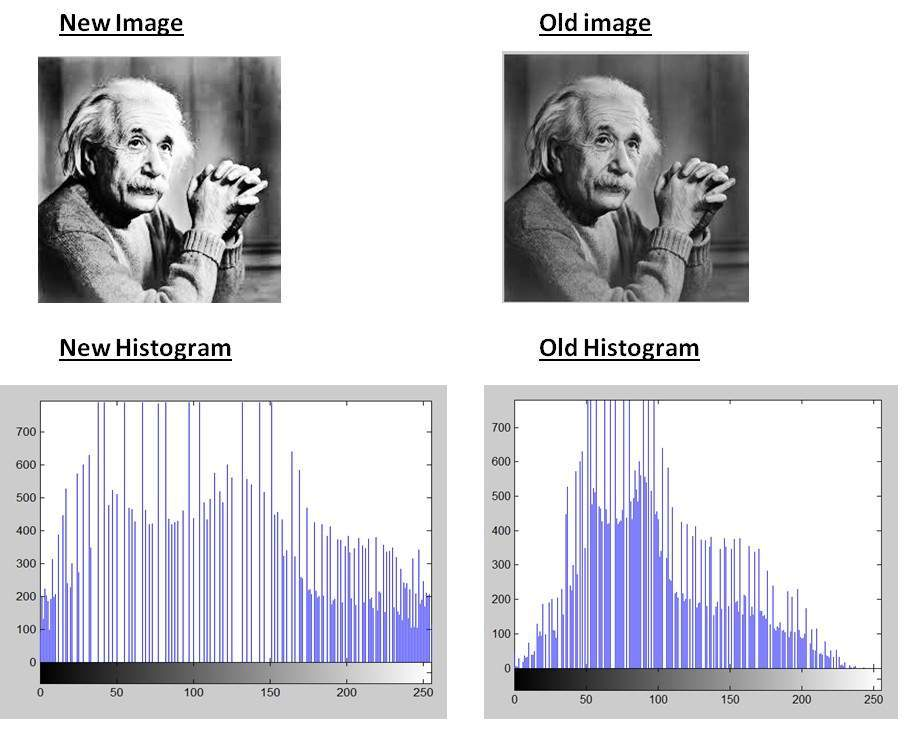
\includegraphics[width=\linewidth]{Bilder/Histogramm}
\setcaptioncitation{https://www.tutorialspoint.com/dip/histogram\_equalization.htm}
\caption{Bearbeitetes Bild mittels Histogram Equalization}
\label{fig:Histogramm}
\end{figure}
Für weitere Anregungen zur Image Pre-Processing Methoden, kann das Journal \textbf{\textit{Preprocessing Technique for Face Recognition Applications under Varying Illumination Conditions}} von \textbf{\textit{Global Journal of Computer Science and Technology Graphics \& Vision}} studiert werden.
\newline
Weshalb wurden diese Methoden nicht verwendet um das Modell zu verbessern? Das Problem liegt in den Rahmenbedingungen. Die Projektmitglieder hatten nicht das Hintergrundwissen wie diese Methoden in dem Modell implementiert werden konnten und waren sich auch nicht der verschiedenen Methoden bewusst. Die Möglichkeiten zur Image Pre-Processing sind derartig Vielzählig und komplex, dass sie in einer eigenen Studienarbeit bearbeitet werden können. Natürlich kann das Modell noch stark verbessert werden durch solche Methoden, doch die definierten Ziele konnten mit der jetzigen Lösung erreicht werden, ohne den zeitlich vorgegebenen Rahmen zu überschreiten.
Doch für eine Weiterentwicklung dieses Modells rentiert es sich, solche Methoden weiter zu studieren und in das Modell mit aufzunehmen.

\section{Reflexion Vorgehen}
\sectionauthor{8774695}

Grundsätzlich wurde das Projekt strukturiert durch die Erstellung, Priorisierung und Abarbeitung von Anforderungen durchgeführt. Auf die Verwendung eines Vorgehensmodelles wurde verzichtet, da zum einen das Projekt aus nur drei Mitgliedern bestand und zum anderen das Umfeld für die Projektmitglieder sehr neu war. Daher war die Planung und Einteilung einzelner Phasen, wie bei dem Wasserfallmodell schwer umzusetzen und hätte keinen deutlichen Mehrwert gebracht. Die Verwendung eines Spiralmodells, wie es in technisch neuartigen Umfeld häufig verwendet wird, war zu schwerfällig und zeitaufwendig. Von daher wurde sich lediglich auf die Definition von Anforderungen gestützt, welche auch erfolgreich umgesetzt wurden. Allerdings stellt sich die Frage, ob die Anforderungen auch korrekt gewählt wurden. Dies soll im folgenden diskutiert werden.
\newline
Anforderungen sollten im Allgemeinen einige Rahmenbedingungen erfüllen, damit sie verständlich und bewertbar sind. Darunter fallen die folgenden Punkte:
\begin{itemize}
\item \textbf{Korrektheit:} Die Anforderung entspricht den Bedürfnissen der Stakeholder.
\item \textbf{Eindeutigkeit:} Die Formulierung der Anforderung erlaubt nur eine gültige Interpretation.
\item \textbf{Prüfbarkeit:} Es lassen sich Kriterien oder Tests angeben, um nachzuweisen, ob die Anforderung erfüllt ist oder nicht.
\item \textbf{Nachverfolgbarkeit:} Der Ursprung der Anforderung und ihre Entwicklung lassen sich feststellen.
\end{itemize}

Zur Bewertung des ersten Punktes, müssen zuerst die Stakeholder des Projektes identifiziert werden. Zu diesen zählen zum einen die Projektbeteiligten und zum anderen dem betreuenden Dozenten. Nachdem die Anforderungen durch alle drei Projektbeteiligten entworfen wurden, kann auf deren Seite eine Korrektheit der Anforderungen bestätigt werden. Mit dem betreuenden Dozenten wurde regelmäßig, vor allem zu Beginn des Projektes, Absprache gehalten. Hierbei wurden die Ziele und Aufgabenstellung des Projektes gemeinsam diskutiert aus welchen auch die Anforderungen hervor gingen. Von daher kann auch von dieser Seite eine Korrektheit der Anforderungen angenommen werden. Schlussfolgernd gilt der erste Punkt als erfüllt.
\newline
In Bezug auf die Eindeutigkeit der Anforderungen, kann man diese für die meisten bestätigen. Allerdings sind vor allem die Anforderungen einer benutzerfreundlichen Interaktionsmöglichkeit und einer Oberfläche zur intuitiven Bedienung stark individuell abhängig. Eine intuitive Bedienung ist für den Techniker schneller gegeben als für den Manager, dessen Erwartungen an solch eine meist höher gesteckt sind. Doch in der frühen Entwicklungsphase wurde sich dafür entschieden diese Anforderungen mit aufnehmen zu müssen, auch wenn es schwierig war die entsprechende Anforderung eindeutig zu beschreiben. Das Problem wurde auch gewitzt umgangen, indem der Anwender gar nicht erst mit der Anwendung interagieren muss.
\newline
Auch für die Prüfbarkeit wurden für die meisten Anforderungen feste Werte oder eindeutige Zeitrahmen definiert um deren Erfüllung bewerten zu können. Aus dem Rahmen fallen auch hier die bereits genannten Anforderungen aus den gleichen Gründen. 
\newline
Bei der Nachverfolgbarkeit muss an dieser Stelle eingestanden werden, dass diese nicht vollständig erfüllt wurde. Der Ursprung der Anforderungen kann auf die ersten Wochen der Bearbeitungszeit festgelegt werden, doch deren genaue Entwicklung ist nicht nach verfolgbar. Der Grund liegt in der fehlenden Dokumentation während dem Entwicklungsverlaufs. Als Dokumentation dient diese Arbeit, jedoch existiert keine genauere Dokumentation, welche Anforderungen an welchen Bearbeitungstagen bearbeitet oder fertig gestellt wurden. Auf diese wurde gezielt verzichtet, da eine Dokumentation einen zusätzlichen Arbeitsaufwand und damit verbunden einen erhöhten Zeitaufwand bedeutet hätte. in einem größeren Team müssen die Tätigkeiten nach verfolgbar sein, da sonst das Scheitern des Projekts möglich ist, doch in diesem Projekt waren lediglich drei Entwickler beteiligt, wodurch auf eine Dokumentation verzichtet werden konnte ohne den Erfolg des Projektes zu gefährden.
\newline
Zuletzt stellt sich die Frage, ob die gegebenen Anforderungen auch vollständig sind. Nach dem aktuellen Kenntnisstand hätten weitere Anforderungen an das Projekt gestellt werden können, wie detailliertere technische Anforderungen im Bezug auf die minimal benötigten Ressourcen der Hardware um nur ein Beispiel zu nennen. Doch zusammenfassend kann gesagt werden, dass die Anforderungen situationsbedingt gut gewählt wurden. Nachdem alle Projektbeteiligten neu in diesem Bereich waren, war es nicht möglich genauere Anforderungen zu stellen, da das entsprechende Wissen fehlte. Die Anforderungen mögen nicht exakt nach der Definition vollständig formuliert worden sein, doch es wurde sich dafür entschieden mit diesen Anforderungen zu arbeiten um ein strukturiertes Vorgehen zu ermöglichen. Bei keiner Vorgabe, wäre die Bewertung eines Erfolgs des Projektes nicht möglich gewesen. 


\section{Reflexion der Literatur}
\sectionauthor{8774695}
Bezüglich der Literatur ergeben sich nun einige Schwierigkeiten. Dies liegt unter anderem daran, dass das generelle Thema der Gesichts und Emotionserkennung immer noch vor allem aus
psychologischer Sicht in der Literatur behandelt wurde. Zwar gibt es Fachbücher auch aus informationstechnischer Sicht, welche ebenfalls in dieser Arbeit verwendet wurden.
\newline
Für die Recherche dieser Arbeit wurden 30 Quellen verwendet, von denen 9 Quellen aus Büchern verwendet wurden und 21 Quellen aus online Recherchen hervorgingen. Die 30\% der schriftlichen Quellen wurden aus Fachbüchern aus diesem Gebiet oder einem verwandten Gebiet des Themas dieser Arbeit verwendet, wodurch eine gute theoretische Einarbeitung in die Thematik ermöglicht wurde. Die Online Quellen wurden größtenteils für technische Lösungsansätze und Bereiche verwendet, welche durch die Fachbücher nicht gedeckt werden konnten. Dabei wurden offizielle Dokumentationen verwendet, die eine optimale Informationsquelle für technische Details der Software bietet, aber nicht für die Bewertung dieser. Diese Dokumentationen wurden jedoch lediglich für technische Hintergrundinformationen verwendet. Des weiteren wurden auch Handbücher und Blogartikel verwendet, welche zwar keine wissenschaftliche Grundlage bieten, aber gute Lösungsansätze für die gestellten Aufgaben anboten. Es wurde im laufe der Arbeit darauf geachtet seriöse und vertrauenswürdige Quellen für die Recherche zu nutzen und keine subjektiven und nicht nach verfolgbaren Verweise in die Arbeit mit einfließen zu lassen.
\newline
Wie eingangs erwähnt, stellt die Recherche von Fachliteratur in Bezug auf Emotionserkennung im technischen Umfeld eine Herausforderung dar. Die schriftlichen Quellen behandeln meist nur die übergeordneten Themen der Künstlichen Intelligenz im Allgemeinen oder mehr in Richtung der Gesichtserkennung. Allerdings waren die Ziele dieser Arbeit mehr praktisch Motiviert und weniger auf die Beantwortung wissenschaftlicher Fragestellungen ausgelegt. Aus diesem Grund gilt die verwendete Literatur als gute Basis für die Erfüllung dieser Arbeit.


\section{Offene Implikationen}
\sectionauthor{8774695}


\section{Alternative Ansätze zur Umsetzung von Emotionserkennung}
\sectionauthor{1329241}
In diesem Abschnitt nun werden verschiedene alternative Ansätze dargestellt und expliziert, die dazu verwendet werden können um Emotionen zu erkennen.
Dieses Unterkapitel beschäftigt sich mit alternativen Ansätzen zu den bereits explizierten Basisemotionen. Diese sind wie bereits erwähnt umstritten, was die Frage zulässt warum diese überhaupt verwendet werden sollten. Alternativen dazu bieten weitere kreative Ansätze, wie die Erkennung von Emotionen anhand der Stimmlage.
Dieser Ansatz beruft sich darauf, dass das Sprachzentrum eines Menschen einer der wichtigsten Aspekte der Kommunikation und somit auch der Preisgabe von Informationen über den emotionalen Zustand eines Individuums ist.
\footcite[Vgl. ][Abstract]{EmotionInSpeech}
Dieser Ansatz ist jedoch nicht zielführend, da hier hauptsächlich die Stimme analysiert wird. Von einer Stimme kann nun auf eine Emotion geschlossen werden. Für den Usecase ist dieser Ansatz allerdings ungeeignet, aus folgenden Gründen:\newline
Es kann möglich sein eine Emotion anhand der Sprache zu erkennen. Das Äquivalent eines Pokerfaces wäre dementsprechend je nach Definition eine neutrale Stimmlage, welche keine Emotionen suggeriert. Nun kann aber keine Aussage getroffen werden aus welchen Gründen eine Person neutral spricht. Es könnte von einem Pokerface stammen, oder einer monotonen Sprechweise, oder einen gelangweilten Gemütszustand. Dies ist nicht eindeutig identifizierbar.
Ein weitere Ansatz wäre die Analyse der derzeit vernommenen Musik. Diese kann einem bestimmten Gemütszustand zugesprochen werden, welches auf eine aktuelle Emotion übertragbar ist.
\footcite[Vgl.][1]{MusicEmotion}
Ziel dieses Forschungszweiges ist es daher die hinter Liedern oder Klängen stehenden Emotionen zu ermitteln und diese entsprechend zu kategorisieren.
Dieser Ansatz erscheint zunächst durchaus interessant, hat jedoch genauso Nachteile wie die Analyse von Emotionen anhand der Stimmlage.
Der Größte liegt hier unter anderem in der Genauigkeit der Analysen. So z.B. lieferte ein Testprojekt an der Russischen HSE (Higher School of Economics) das Ergebnis von einer maximalen Genauigkeit von 71\%.
\footcite[Vgl. ][Abstract]{EmotionInSound}
In dem Versuchsaufbau wurden Spektrogramme von Klangfragmenten ausgewertet und versucht mittels Neuronalen Netzen eine Klassifikation der hinter dem Klang liegenden Emotion zu erreichen.
\footcite[Vgl. ][Abstract]{EmotionInSound}
Der generelle Ansatz anhand von Musik die Emotion eines Individuums abzulesen ist zwar praktikabel und von dem Versuchsaufbau auch vergleichbar zu dem Ansatz bereits gelabelte Bilder zu verwenden. Jedoch lässt sich auf diese Weise aus zwei Gründen nicht die eigentliche Zielaufgabenstellung ableiten - das Erkennen eines Pokerfaces. Zum einen handelt es sich in dieser Arbeit um eine visuelle Problemstellung, in welcher das Erkennen des Gemütszustandes anhand des Gesichtsausdruckes erkannt werden soll, also einem vorhandenen bzw. nicht vorhandenen Pokerface. Zum anderen würde die Analyse von Musik einen Rückschluss auf den allgemeinen Gemütszustand des Betroffenen folgern und nicht eine kurzzeitige Stimmungsschwankung aufgrund beispielsweise eines schlechten Kartenblattes. \newline
Anhand der hier gezeigten Alternativen kann Emotionsanalyse auf verschiedenste Weise implementiert werden. Die Pokerface-Erkennung hingegen kann lediglich visuell erfolgen, weshalb die hier explizierten Ansätze dafür nicht valide sind.

\let\cleardoublepage\relax
\newpage
\printbibheading
\thispagestyle{empty}
\pagestyle{empty}
\printbibliography[type=book,heading=subbibliography,title={Literaturquellen}]
\newpage
\printbibliography[type=misc,heading=subbibliography,title={Sonstige Quellen}]
\newpage


%\begin{appendix}
%\renewcommand\thefigure{{App}.\Alph{figure}}
%\renewcommand\thetable{{App}.\Roman{table}}
%\renewcommand\thelstlisting{{App}.\arabic{lstlisting}}
\chapter*{Anhang}
\thispagestyle{empty}
\section*{Verwendeter Code}
  
  \lstinputlisting[style=custompython, caption=Code für GUI mit Video Stream der Webcam als Output, label=lst:Code Input GUI 1]{Code/InputGUI1.py}
  \newpage
  \lstinputlisting[style=custompython, caption=Code für GUI mit Video Stream der Webcam und markierten Gesichtern als Output, label=lst:Code Input GUI 2]{Code/InputGUI2.py}
  \newpage
  \lstinputlisting[style=custompython, caption=Code für GUI mit Video Stream der Webcam und markierten Gesichtern und Augen als Output, label=lst:Code Input GUI 3]{Code/InputGUI3.py}
  \newpage
  \lstinputlisting[style=custompython, caption=Dataset sortieren und überarbeiten, label=lst:Organising The Dataset]{Code/OrganizingTheDataset.py}
  \newpage
  \lstinputlisting[style=custompython, numbers=none, linerange=8-17, caption=Trainingsdaten als Arrays extrahieren, label=lst:Trainingsdaten extrahieren]{Code/ClassifierHandler.py}
  \newpage
  \lstinputlisting[style=custompython, caption=Skript zum Trainieren und Testen eines FisherFaceRecognizer, label=lst:Classifier Handler]{Code/ClassifierHandler.py}
  \newpage
  \lstinputlisting[style=custompython, numbers=none, linerange=26-50, caption=Klassifizierer mit der Input GUI testen, label=lst:Text mit Input GUI]{Code/ClassifierHandler.py}
  \newpage
\section*{Verzeichnisstrukturen}
\setlength{\DTbaselineskip}{20pt}
\DTsetlength{1em}{1.5em}{0.2em}{1pt}{4pt}
\renewcommand*\DTstylecomment{\rmfamily\color{commentgreen}\textsc}
\renewcommand*\DTstyle{\ttfamily\textcolor{red}}
\begin{figure}[h]
\begin{minipage}[b]{.5\linewidth}
\dirtree{%
.1 images.
.2 S005\DTcomment{Person 1}.
.3 001.
.2 S010\DTcomment{Person 2}.
.3 001.
.3 002.
.3 003.
.2 S011\DTcomment{Person 3}.
.3 001.
.3 002.
.2 S014\DTcomment{Person 4}.
.3 001.
.3 002.
.3 003.
.3 004.
.3 005.
.2 \ldots.
}
\end{minipage}
\begin{minipage}[b]{.5\linewidth}
\dirtree{%
.1 emotions.
.2 S005\DTcomment{Person 1}.
.3 001.
.2 S010\DTcomment{Person 2}.
.3 001.
.3 002.
.3 003.
.2 S011\DTcomment{Person 3}.
.3 001.
.3 002.
.2 S014\DTcomment{Person 4}.
.3 001.
.3 002.
.3 003.
.3 004.
.3 005.
.2 \ldots.
}
\end{minipage}
\caption{Verzeichnisstrukturen des Cohn-Kanade Datasets}
\label{fig:Struktur CK Dataset}
\end{figure}

\begin{figure}
	\dirtree{%
	.1 sorted\_set.
	.2 anger.
	.3 1.png.
	.3 2.png.
	.3 \ldots.
	.2 contempt.
	.3 1.png.
	.3 2.png.
	.3 \ldots.
	.2 disgust.
	.3 1.png.
	.3 2.png.
	.3 \ldots.
	.2 fear.
	.3 1.png.
	.3 2.png.
	.3 \ldots.
	.2 happy.
	.3 1.png.
	.3 2.png.
	.3 \ldots.
	.2 neutral.
	.3 1.png.
	.3 2.png.
	.3 \ldots.
	.2 sadness.
	.3 1.png.
	.3 2.png.
	.3 \ldots.
	.2 surprise.
	.3 1.png.
	.3 2.png.
	.3 \ldots.
	}
\caption{Struktur überarbeitetes Dataset}
\label{fig:Tree Sorted Set}
\end{figure}
\section*{Sonstiges}
\begin{figure}[h]
  \center
  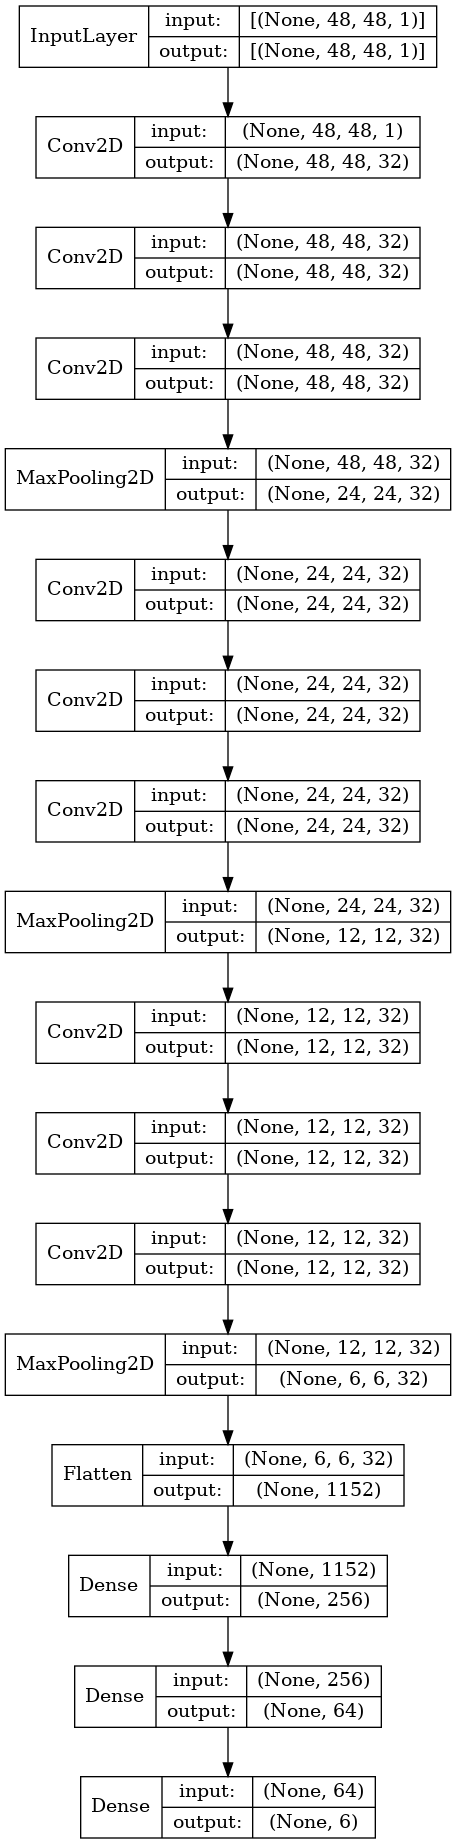
\includegraphics[scale=0.35]{Bilder/ModelSummary.png}
  \caption{ Model Summary with several Layers and I/O Shapes }
  \label{fig:Model Summary}
  \end{figure}
%\end{appendix}
\end{document}
